% Project Task 2: model transformation
% Model Driven Engineering, University of Twente
%
% Always compile twice, to get the table of contents and references right.
\documentclass[10pt, a4paper, oneside]{article}
\usepackage[left=2cm, right=2cm, top=2.5cm, bottom=3cm]{geometry}
\usepackage{color}          % So you can use colors
\usepackage{amsmath}        % For all kinds of math symbols
\usepackage{graphicx}       % Package to include photos and graphs
\usepackage{float}          % Helps in positioning floats
\usepackage[justification=centering]{caption}  % To center the captions
\usepackage{url}
\usepackage{xcolor}
\usepackage{hyperref}
\usepackage{tabularx}
\usepackage{longtable}
\usepackage{booktabs}
\usepackage[T1]{fontenc}
\usepackage{textcomp}
\usepackage{listings}
\usepackage{nameref}
\usepackage{pdflscape}
\renewcommand{\lstlistingname}{Example}  % a listing is called an Example here

% Code listings, coloured by language with listings alone: the Overleaf
% instance runs without shell escape, so minted and Pygments are not an option.
\definecolor{codebg}{HTML}{F8FAFC}
\definecolor{codeframe}{HTML}{CBD5E1}
\definecolor{codekey}{HTML}{1E40AF}
\definecolor{codeattr}{HTML}{7C3AED}
\definecolor{codestring}{HTML}{047857}
\definecolor{codecomment}{HTML}{64748B}
\definecolor{codeliteral}{HTML}{B45309}
\lstdefinestyle{report}{
  backgroundcolor=\color{codebg}, frame=single, rulecolor=\color{codeframe},
  framesep=4pt, xleftmargin=5pt, xrightmargin=5pt, captionpos=b,
  basicstyle=\normalsize\ttfamily, columns=fullflexible, keepspaces=true,
  breaklines=true, showstringspaces=false,
  commentstyle=\color{codecomment}\itshape, stringstyle=\color{codestring},
  keywordstyle=\color{codeliteral}}
% YAML: a line starts as a key, and turns into a value at its first colon.
\newcommand\yamlkey{\color{codekey}\normalsize\ttfamily}
\newcommand\yamlvalue{\color{black}\normalsize\ttfamily}
\newcommand\yamlcolon{\color{black}}
\lstdefinelanguage{yaml}{
  basicstyle=\yamlkey, keywords={true,false,null},
  keywordstyle=\color{codeliteral}, sensitive=true,
  comment=[l]{\#}, morestring=[b]', morestring=[b]",
  moredelim=**[il][\yamlcolon{:}\yamlvalue]{:},
  literate={-\ }{{\color{black}-\ }}2}
% QVT Operational Mappings: the keywords the listings use.
\lstdefinelanguage{qvto}{
  morekeywords={modeltype,uses,transformation,in,out,access,library,import,
    configuration,property,main,mapping,query,init,end,object,var,let,if,then,
    else,elif,endif,and,or,not,self,result,map,resolveone,assert,fatal,with,
    log,return,disjuncts,Sequence,Tuple},
  keywordstyle=\color{codekey}\bfseries, sensitive=true,
  comment=[l]{--}, morestring=[b]'}
\lstdefinelanguage{ocl}{
  morekeywords={context,inv,def,let,in,if,then,else,endif,implies,and,or,not,self},
  keywordstyle=\color{codekey}\bfseries, sensitive=true,
  comment=[l]{--}, morestring=[b]'}
\setlength{\parindent}{0pt} % When you do not want indentation for your paragraphs.
\setlength{\parskip}{5pt}   % For space between paragraphs.
\setlength{\emergencystretch}{2em} % let a line with a long code word stretch rather than overrun

\hypersetup{
  colorlinks=true,
  linkcolor=blue!55!black,
  citecolor=blue!55!black,
  urlcolor=blue!55!black,
  linktoc=all,
  bookmarksnumbered=true,
}

% Heading and list layout. This is a short report, so the headings stay small
% and the spacing around them tight. The Overleaf instance carries no titlesec
% or enumitem, so both are reproduced with the kernel's own commands.
\makeatletter
\renewcommand\section{\@startsection{section}{1}{\z@}%
  {-2.2ex \@plus -0.6ex \@minus -.2ex}{0.6ex \@plus.2ex}%
  {\normalfont\large\bfseries}}
\renewcommand\subsection{\@startsection{subsection}{2}{\z@}%
  {-1.8ex \@plus -0.5ex \@minus -.2ex}{0.4ex \@plus.2ex}%
  {\normalfont\normalsize\bfseries}}
\def\@listI{\leftmargin\leftmargini
  \parsep 0pt \topsep 3pt \itemsep 1pt}
\let\@listi\@listI
\makeatother

\begin{document}
%==== FRONT PART====
\begin{titlepage}

\newcommand{\HRule}{\rule{\linewidth}{0.5mm}}
\begin{center}
~\vspace{2cm}

\HRule \\[0.6cm]
\textbf{\LARGE Resolving Project Intent into a Kubernetes Deployment Model} \\[0.3cm]
Project Task 2: Model Transformations \\
Project Type: Code Generation \\
October 16, 2026\\[0.4cm]
\HRule \\[1.2cm]
\text{\large Joris Jonkers (s1829157)}\\[0.4cm]
\text{\large Model Driven Engineering}\\
\text{\large University of Twente}\\
\end{center}
\newpage
\end{titlepage}

\pagenumbering{roman}
\tableofcontents

%==== MAIN PART ====
\newpage
\pagenumbering{arabic}
\section{Purpose of the Project}
\label{sec:purpose}

\subsection{Goals}
\label{sec:goals}

The project converts short deployment documents into Kubernetes files for an
existing small cluster. Each project repository holds one
\texttt{Project Intent} document. This document describes its \texttt{Application}s, including their \texttt{Process}es, memory and CPU limits, ports, dependencies, and external routes. One \texttt{Platform Intent} document defines shared
policies and resources, including cluster entry points, health-check timings,
and backup policies. Task~1 defined two Ecore metamodels: a source metamodel
for the authored documents and a target metamodel for the
\texttt{Resolved Deployment}. The target model records the values derived for
each \texttt{Application} and the paths of the files to be generated.

Task~2 implements the transformation to \texttt{Resolved Deployment}.
It combines all authored models with recorded cluster facts, image digests,
and other pinned inputs, producing one resolved model per \texttt{Project}.
For example, an image name becomes a repository address pinned to a digest,
and a dependency declaration becomes a host-and-port combination. Task~3 then
generates files from these resolved values.

\begin{table}[!htbp]
\centering
\begin{tabular}{>{\raggedright\arraybackslash}p{0.2\linewidth}>{\raggedright\arraybackslash}p{0.72\linewidth}}
\hline
\textbf{Term} & \textbf{Meaning} \\
\hline
\texttt{Process} & One program of an \texttt{Application}, running in its own pods. \\
\texttt{Dependency edge} & A declaration by one \texttt{Process} that it calls a named port of another \texttt{Application}. \\
\texttt{Pinned input set} & The read-only inputs besides authored documents: node contract (machines and capacity), images lock (image digests), \texttt{ClusterState} snapshot, migration proofs, and configuration-file contents. \\
\texttt{Asset} & A configuration file mounted into a \texttt{Process}. \\
\texttt{Exposure} & An external address and routes to an \texttt{Application}'s ports. \\
\texttt{Switchover} & How a new version replaces the old: blue/green (both versions run simultaneously, and traffic switches to the new once it is healthy), rolling (gradual replacement), or stop-start (old stops before new starts). \\
\texttt{ReleaseGate} & The resolved configuration for the service that blocks a blue/green switch until the \texttt{Application}'s \texttt{Process}es are healthy, preventing traffic from reaching an unhealthy version. \\
\texttt{ReconcileUnit} & A group of resources that Flux (the GitOps operator) reconciles together as a unit, with dependencies on other such groups. \\
\texttt{Entry point} & A platform listener (class \texttt{Tier} in the source metamodel) that admits specified audiences and forwards routes through a proxy. \\
\texttt{Revision} & A release identifier computed by hashing an \texttt{Application}'s resolved configuration. \\
\texttt{Estate} & All \texttt{Project}s, the \texttt{Platform Intent}, and the \texttt{Pinned input set} read by one run. \\
\texttt{Flattened model} & \texttt{Project Intent} with every shared declaration copied down onto the \texttt{Process}es that reference it (class \texttt{EffectiveProject}), preserving declaration precedence. \\
\hline
\end{tabular}
\caption{Project Terms Used in This Report}
\label{tab:terms}
\end{table}

\paragraph{Design Approach.} The transformation is deterministic: the same
pinned inputs always produce the same resolved model, with no reads of live
cluster state. Every value the Task~3 templates need is recorded in the
resolved model itself, so template tests cannot pass while a template makes an
unchecked deployment decision. Where a value cannot be derived, the run aborts
with an error message rather than fabricating a default: a missing or
fabricated value could otherwise produce a valid-looking file that deploys
the wrong configuration. Conformance to the specification's oracle files is
verified by byte-exact comparison of resolved values, dependency edges,
generated files, JSON, and release digests (Section~\ref{sec:evaluation}).

\subsection{Role of the Transformations}
\label{sec:role}

Figure~\ref{fig:pipeline} shows the pipeline. Xtext converts each document
to a source model, and the Task~1 OCL constraints reject invalid ones. Three
QVT-Operational transformations (QVTo) then run in sequence.

The first transformation, the flattening, copies declarations made once for an
entire \texttt{Project} or \texttt{Application} down onto each \texttt{Process}.
Its output is the flattened model, which still conforms to the
source metamodel. Although it was implemented in Task~1, it was not reported
there, so Section~\ref{sec:flattening} covers it here. The second
transformation, the resolution, reads the flattened models and the
\texttt{Pinned input set}, the additional read-only inputs, and derives
one complete \texttt{Resolved Deployment} per
\texttt{Project}. It is the main transformation and the subject of this
report. The third, the final pass, collects Vault policies from all resolved
models to plan one job that installs them in Vault, the platform's secret
management service. This requires every \texttt{Project}'s
output, so it runs after the individual resolutions (Section~\ref{sec:finalpass}).

A small Java exporter writes the resolved dependency edges as JSON for
comparison against the oracle. The Acceleo templates of Task~3 then read the
\texttt{Resolved Deployment}s and generate the Kubernetes files.

\begin{figure}[!htbp]
\centering
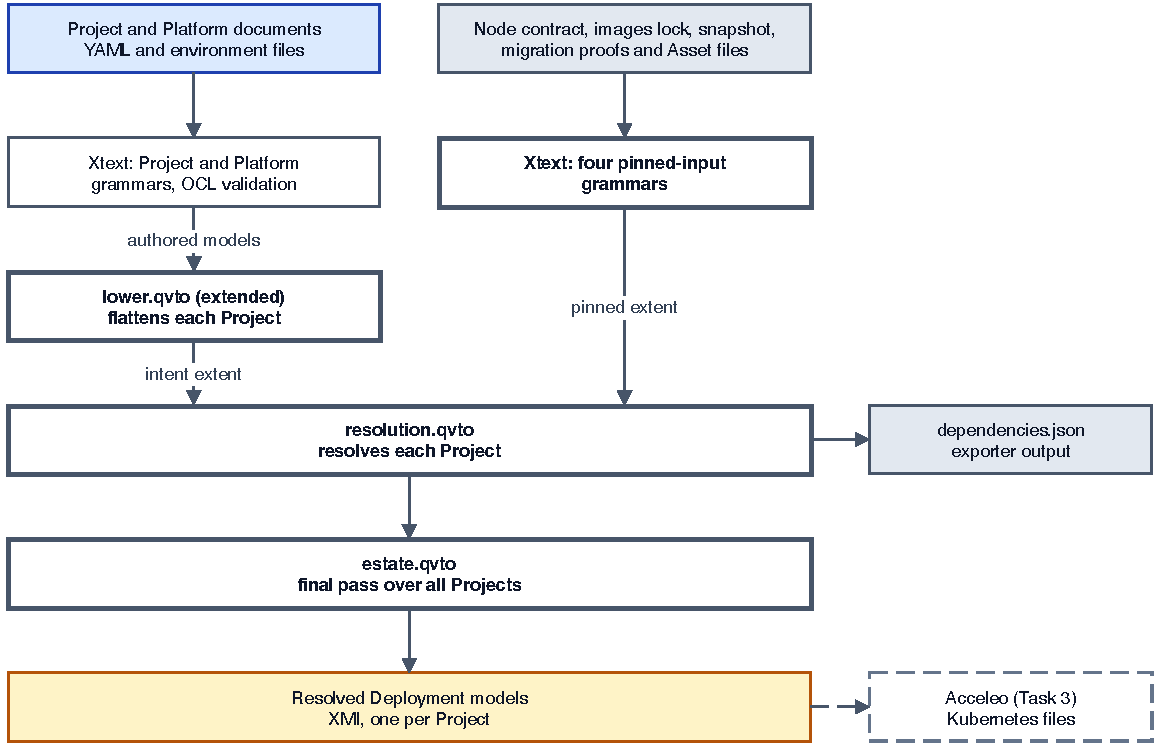
\includegraphics[width=\linewidth, keepaspectratio]{Figures/pipeline}
\caption{The Pipeline, With What Task~2 Added or Extended in Bold}
\label{fig:pipeline}
\end{figure}

\subsection{Refinement of Tasks 0 and 1}
\label{sec:refinement}

Task~0 treated the node contract (the list of machines and their capacity),
the images lock (each image pinned to a digest), and the \texttt{ClusterState} snapshot
as plain inputs, while Task~1 only
modelled the two authored documents. The resolution needs these as models, so
a third metamodel now describes the \texttt{Pinned input set}, with its own
Xtext grammar for each document (Appendix~\ref{app:pinned}). A separate
package keeps these supporting inputs distinct from the deployment language
used by \texttt{Project} authors.

Task~1 described three stages: authored, resolved, and generated text. The
flattening now resolves shared declarations before resolution: each
\texttt{Process} receives the declarations that apply to it from its
\texttt{Project} and \texttt{Application}. Resolution rules therefore need
not repeat that merge logic (Section~\ref{sec:twotransformations}).

Task~1 planned one resolved model for the entire cluster, because resolving
dependency edges, routes, and network access requires a cluster-wide view.
Every run still reads every \texttt{Project}. The output is now one
\texttt{Resolved Deployment} per \texttt{Project}, because each model then
stays small and has one oracle to compare with
(Section~\ref{sec:perproject}). Each \texttt{Application} still has its own
\texttt{ResolvedApplication} inside that
model. The final pass adds the one job that no single \texttt{Project}'s resolution
can compute (Section~\ref{sec:finalpass}).

Task~1 demonstrated the target metamodel with only the \texttt{minimal} example. The
other examples needed additional concepts: migrations, backup service accounts, API
access, sidecar containers, and twelve additional file types (see Appendix~\ref{app:metamodels} for the complete list).

\subsection{Assumptions and Scope}
\label{sec:scope}

The transformation assumes four conditions.

\begin{itemize}
  \item \textbf{Checked input.} The OCL constraints check the authored documents
    before transformation begins. Aborts reject invalid inputs that these
    constraints do not yet catch (Section~\ref{sec:aborts}).
  \item \textbf{One cluster per run.} Each execution of the pipeline reads
    all documents for one cluster, including one \texttt{Platform Intent}
    and one node contract that name the same cluster. All concepts,
    examples, and oracles derive from that single existing cluster.
  \item \textbf{One reading of the specification.} If several providers
    satisfy a dependency, the transformation uses the deterministic name
    order recorded in the oracles. The comparisons check this interpretation, but
    they do not establish that it is the only valid one.
  \item \textbf{No live cluster access.} The transformation only reads the
    documents provided to it. Any fact known only to a running cluster, such
    as which node holds a particular volume, must arrive via the
    \texttt{ClusterState} snapshot captured by another process.
\end{itemize}

\paragraph{More Than One Cluster.} A second cluster would need a separate
run with its own \texttt{Platform Intent}, node contract, and
\texttt{ClusterState} snapshot. Environment-specific configuration overlays are already selected
by cluster name (Section~\ref{sec:placeholders}). The model would also need
to declare which clusters each \texttt{Project} targets and to represent
cross-cluster network access with address ranges. Such dependencies could
use the external-provider mechanism (Section~\ref{sec:edgerule}), already used by the \texttt{auth} \texttt{Project} for its
mail server. This extension has not been implemented.

Table~\ref{tab:scope} sets the scope of Task~2.

\begin{table}[!htbp]
\centering
\begin{tabular}{>{\raggedright\arraybackslash}p{0.46\linewidth}>{\raggedright\arraybackslash}p{0.46\linewidth}}
\hline
\textbf{In scope} & \textbf{Out of scope} \\
\hline
The resolution of eight examples: \texttt{minimal}, \texttt{auth},
  \texttt{data}, \texttt{delivery}, \texttt{edge},
  \texttt{knowledge-platform}, \texttt{observability}, and \texttt{secrets}. &
  The \texttt{knowledge} example, which is being retired with its
  project and is excluded from this test set (Section~\ref{sec:limitations}). \\
Every derivation these examples use, from dependency edges and placement to
  backups, migrations, network peers, and the path of every generated file. &
  The text of the generated files, which is Task~3. \\
The flattening's extensions, the final pass, and the \texttt{Pinned input set} metamodel
  and grammars. &
  Applying files to a running cluster (Task~3 responsibility) or targeting multiple clusters (not supported by current design). \\
\hline
\end{tabular}
\caption{Scope of Task 2}
\label{tab:scope}
\end{table}

\section{Alternatives and Justification}
\label{sec:alternatives}

\subsection{Existing Kubernetes Modelling Tools}
\label{sec:existingtools}

Three open-source tools were reviewed to see whether they could produce the
\texttt{Resolved Deployment} from \texttt{Project Intent} and
\texttt{Platform Intent}, or at least take part in the pipeline.
Table~\ref{tab:tools} compares them.

\begin{table}[!htbp]
\centering
\begin{tabular}{>{\raggedright\arraybackslash}p{0.15\linewidth}>{\raggedright\arraybackslash}p{0.24\linewidth}>{\raggedright\arraybackslash}p{0.24\linewidth}>{\raggedright\arraybackslash}p{0.24\linewidth}}
\hline
\textbf{Tool} & \textbf{What it does} & \textbf{Why it cannot replace the resolution} & \textbf{Where it could help} \\
\hline
KubeDiagrams \cite{kubediagrams} &
  Draws diagrams from Kubernetes files or a live cluster, mapping kinds to icons. &
  It needs Kubernetes resources as input, so it cannot derive them from deployment intent. &
  It could visualize the generated files to show links produced by a \texttt{Project} document. \\
KubeOrch \cite{kubeorch} &
  A drag-and-drop editor whose back end wires ports, fills templates, writes files and deploys. &
  It has no metamodel and no constraints; its rules are Go code, and it deploys directly, not via Flux. &
  Its graph notation could inform a \texttt{Project} document editor. \\
kubert \cite{kubert} &
  A command-line tool to switch cluster contexts and run commands on multiple clusters. &
  It is an operations tool and does not model or generate anything. &
  It could apply files to several clusters, which is out of scope. \\
\hline
\end{tabular}
\caption{Existing Kubernetes Modelling Tools}
\label{tab:tools}
\end{table}

None of the three derives values from authored declarations. KubeOrch
comes closest: it resolves a link between two services to an address and
port, similarly to the dependency-edge lookup in this project.
But it lacks a \texttt{Platform Intent}, node contract,
images lock and cluster-state snapshot, so it cannot derive placement, image
digests, backups or the connections permitted by network policies. It also
provides no resolved intermediate model to check before generating files.
KubeDiagrams could complement the
transformation by visualizing the Task~3 files, allowing the resolved
dependencies and network connections to be inspected. A
KubeOrch-style graphical editor
could write \texttt{Project Intent} documents, since the editor and the
transformation would work from the same Ecore metamodel.

\subsection{The Transformation Language}
\label{sec:language}

Four languages were considered: ATL, QVT-Relations, QVT-Operational (QVTo) and
Java with a rule library such as SiTra.

QVT-Relations was ruled out first. Its automatic traces and two-way
synchronisation offer no benefit for a one-way derivation. In the cited
experiments, one of its engines, medini QVT, ran into heap-space problems
and became unresponsive on general-case input models with more than a
hundred classes or a hundred attributes~\cite{amstel2011}.

ATL, QVTo and Java were compared against the specific needs of this
transformation. Most values in a \texttt{Resolved Deployment} do not derive
from a single source element: a \texttt{Process}'s eligible machines depend on the
node contract, a route's precedence on other routes, and a \texttt{Process}'s ingress
peers on every \texttt{Process} in the cluster that depends on it. ATL's matched rules
fit one source element producing one target element, with the engine
choosing the order. Here, dependency lookup must search across
\texttt{Project}s, and a \texttt{Revision} can be computed only after its
\texttt{Application} has been assembled. ATL would still need helpers and
explicit calls for these operations. Matched rules alone would therefore
not remove the need to coordinate the transformation's execution.

A Java transformation would be the easiest to debug and offers full
control, but it requires maintaining the trace by hand and hides the
transformation rules inside general-purpose code; some attendees of the
cited discussion called model management in such code hard to
maintain~\cite{burgueno2019}.

QVTo was chosen because these dependencies can be expressed directly:
map the \texttt{Process}es before building routes that refer to them, then
compute the \texttt{Revision} in an \texttt{end} section after the model is
complete. Its trace lets a route find the resolved \texttt{Process} created
from its source reference. OCL also allows the existing constraint vocabulary
to be reused for lookups across the input models. Among the cited survey's respondents it was the
second most-used transformation language after ATL, and its users named its
maturity and its support by a standard as reasons to use
it~\cite{burgueno2019}. The one operation QVTo cannot express directly,
computing a SHA-256 hash, uses QVT's black-box mechanism: a Java library
called through a contextual operation (Section~\ref{sec:blackbox}).

Speed was not a factor. The transformation is a proof of concept: it serves
to work out the complete design and to check it against the specification's
examples, not to run the cluster in the long term. The compiler is to be
ported to a general-purpose language, such as TypeScript or, in the long term,
Rust. Whether the cluster has enough capacity to host the applications is a
separate limitation, discussed in Section~\ref{sec:limitations}.

\subsection{The Structure of the Transformation}
\label{sec:structure}

Every derived value must be recorded in a model before code generation.
This allows tests to compare the values with the oracles independently of
the templates that write them to files.

\subsubsection{Flattening Before the Resolution}
\label{sec:twotransformations}

A single transformation from authored model to \texttt{Resolved Deployment}
would work, but a flattening precedes the resolution. The flattening copies
shared declarations down to each \texttt{Process}. For example, a
\texttt{Project} startup budget of 30s reaches every \texttt{Process}
except one that declares a more specific value, such as 20s. Resolution can
then read the selected budget directly from each \texttt{Process}, without
searching its ancestors. The chain also matches QVT
specification Section~8.1.13, which composes a preparation transformation
before the main one~\cite{qvt13}.

\subsubsection{Resolving One Project with All Projects as Input}
\label{sec:perproject}

One resolution over all \texttt{Project}s at once could produce one
\texttt{Resolved Deployment} for the whole estate. Instead, each invocation
resolves one \texttt{Project} into its own model while reading every
\texttt{Project}'s documents from the same input extent. Each model stays small and
can be compared with its own oracle, while the shared extent provides the
cluster-wide view needed to resolve dependencies, routes and network access. One
value, the digest over all Vault documents, needs the output of every
\texttt{Project}, so the final pass, which runs over all resolved models together,
adds it (Section~\ref{sec:finalpass}).

\subsubsection{Typed Extents}
\label{sec:extentsalternative}

A rule also has to find the run's other documents. Using OCL's
\texttt{allInstances()} would search the loaded models on each evaluation,
making the search scope depend on which files had been loaded. Instead, the
transformation selects each input once by type from two extents that hold
exactly the run's documents, and every rule navigates from one of these
properties (Section~\ref{sec:interface}).

\subsubsection{Aborts, Not Defaults}
\label{sec:abortsalternative}

A default for a value the resolution cannot derive would give a file that
looks valid and deploys the wrong configuration, so the run aborts instead,
through a fatal assertion in an abort query (Section~\ref{sec:aborts}). The
caller then has to handle the failure.

\section{Solution Design}
\label{sec:design}

The resolution is one QVTo transformation, \texttt{resolution.qvto}, of about
1700 lines: 8 mapping operations and 140 queries. The estate pass,
\texttt{estate.qvto}, adds about 130 lines, and the lowering,
\texttt{lower.qvto}, about 340. This section first classifies the three and
describes the lowering (Section~\ref{sec:lowering}), then the resolution's
interface (Section~\ref{sec:interface}), the division into mappings and queries
(Section~\ref{sec:shape}), a worked example (Section~\ref{sec:worked}), the
derivation rules (Section~\ref{sec:rules}), the trace and late assignment
(Section~\ref{sec:trace}), the black-box library (Section~\ref{sec:blackbox}),
the estate pass (Section~\ref{sec:estatepass}), the stops
(Section~\ref{sec:stops}), and how the transformations are run
(Section~\ref{sec:running}).

Figure~\ref{fig:pattern} shows which metamodels the resolution and the estate
pass read and write; each transformation names them in \texttt{modeltype}
declarations, by their namespace URI. The three transformations differ in kind,
and each kind was chosen for its job. All three are one-way:

\begin{itemize}
  \item the \emph{lowering} is endogenous and horizontal: it reads and writes
    the source metamodel, at the same level of abstraction, into a new model
    (out-place), one project in, one out;
  \item the \emph{resolution} is exogenous and vertical, a refinement that adds
    platform detail: it reads the source and pinned-inputs metamodels and
    writes the target metamodel, many models in (N), one out (1);
  \item the \emph{estate pass} is endogenous and in-place: it updates the
    resolved models of a run through an \texttt{inout} extent (M to N).
\end{itemize}

\begin{figure}[!htbp]
\centering
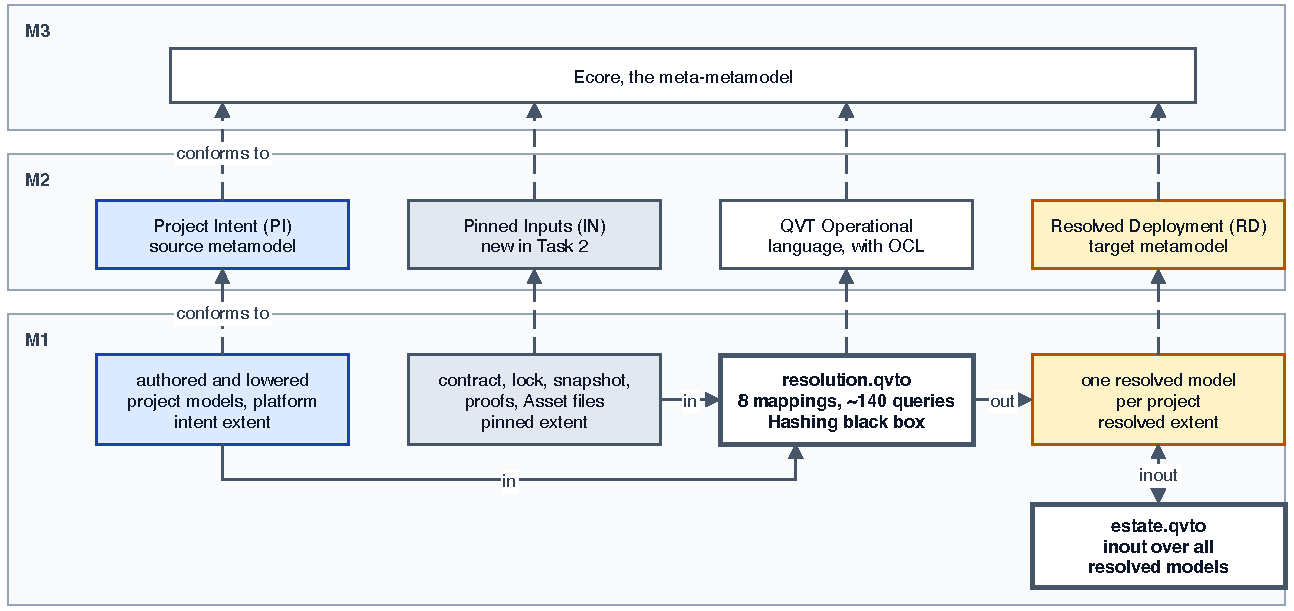
\includegraphics[width=0.85\linewidth, keepaspectratio]{Figures/pattern}
\caption{The Resolution and the Estate Pass in the Metamodel-Based Transformation Pattern}
\label{fig:pattern}
\end{figure}

\subsection{The Lowering}
\label{sec:lowering}

The lowering, \texttt{lower.qvto}, turns each authored \texttt{Project} into an
\texttt{EffectiveProject}, in which every process carries all the shared
declarations that apply to it and the project and applications carry none. It
was part of the Task~1 implementation; Task~2 extended it with API access and
engine grants. It has 37 small mappings, nearly all copies, and three merge
rules:

\begin{itemize}
  \item a list (secrets, dependency edges, Assets, environment entries) is
    the union of the three levels, keyed by each item's own identity, and the
    lowest level that declares an item wins;
  \item a single value (a startup budget, a cutover) comes from the lowest level
    that declares it;
  \item memory and CPU come only from the process itself.
\end{itemize}

Two details are specific to QVTo. A mapping returns its cached result when it
is called again on the same source, so a declaration shared by three processes
would become one object that the last process takes into its containment. Every
shared copy is therefore a mapping with the process as a parameter
(\texttt{copyFor(self)}), which keys the trace on the pair. And a migration is
one of three subclasses, so its copy is a \texttt{disjuncts} mapping that
selects the subclass at run time. The lowering has no stops: the constraints run
before it, so every input it sees is valid.

\subsection{Interface}
\label{sec:interface}

Example~\ref{lst:header} shows the signature. The resolution reads two
\emph{extents}, the sets of models a transformation is given, of two
metamodels, and writes one extent of a third.

\begin{lstlisting}[language=qvto, style=report, caption={The Signature and Inputs of the Resolution, Abridged}, label={lst:header}]
transformation resolution(in intent : PI, in pinned : IN, out resolved : RD)
	access library Hashing;
configuration property project : String;    -- the project this run resolves
property estate : Platform = intent.rootObjects()[Platform]->any(true);
property projects : Sequence(EffectiveProject) =
	intent.rootObjects()[EffectiveProject]->sortedBy(p | p.project)->asSequence();
property lock : ImagesLock = pinned.rootObjects()[ImagesLock]->any(true);
-- and likewise contract, snapshot, proofs and assetFiles
main() {
	projects->select(p | p.project = project)->any(true).map deployment();
}
\end{lstlisting}

The \texttt{intent} extent holds, for every project of the run, its authored
model and its lowered model (\texttt{Effective\-Project}), and the platform
document. The authored models stay in the extent only because the platform
document refers into them: an entry point names the proxy application that
serves it, as an Ecore reference. Every rule reads the lowered models. The
\texttt{pinned} extent holds the node contract, the images lock, the snapshot,
each project's migration proof, and one \texttt{AssetFile} per configuration
file. Two configuration properties give what is not derived: the project to
resolve, and the integrity digest of the schema package, which the resolved
model records as provenance.

The properties select each input once, by type, from the roots of its extent.
This is the only way the transformation reaches other documents: every rule
navigates from one of the seven properties, and no rule calls
\texttt{allInstances()}.
A query over ``every process in the cluster'' is
\texttt{projects.applications.processes}, whose extent is exactly the run's
documents. The projects are sorted by name, so that ``the first provider'' of a
service is the same in every run and in both implementations.

\subsection{Mappings and Queries}
\label{sec:shape}

QVTo offers two ways to create a target object. A \emph{mapping operation}
records its source and result in the trace, the record of which target object
was made from which source. Other rules find the result later with
\texttt{resolveone}, and calling the mapping twice on the same source returns
the same result. \emph{Object creation} (an \texttt{object} expression) inside
a query makes an object that no other rule needs to find. The transformation
uses a mapping exactly where another rule refers to the result, and object
creation everywhere else. Each target type has exactly one mapping, so the
type alone identifies the result: \texttt{p.resolveone(ResolvedProcess)} needs
no \texttt{resolveIn}. No mapping has a \texttt{when} guard or inherits from
another: the caller selects what to map with \texttt{->select}, which keeps the
choice in one visible place. Table~\ref{tab:mappings} lists the eight mappings.

\begin{table}[!htbp]
\centering
\begin{tabular}{>{\raggedright\arraybackslash}p{0.33\linewidth}>{\raggedright\arraybackslash}p{0.59\linewidth}}
\hline
\textbf{Mapping} & \textbf{What it creates, and why it is a mapping} \\
\hline
\texttt{EffectiveProject::\allowbreak deployment} &
  The \texttt{ResolvedDeployment}. Its \texttt{end} section sets the values that
  need the complete model. \\
\texttt{EffectiveProject::\allowbreak unit} &
  The project's reconcile unit, the group Flux applies together. Each
  application refers to it. \\
\texttt{EffectiveProject::\allowbreak provenance} &
  The digest of every input and the hash over them; its \texttt{end} section
  takes the hash. \\
\texttt{EffectiveApplication::\allowbreak application} &
  A \texttt{ResolvedApplication}. Generated files and the revision refer to it. \\
\texttt{EffectiveApplication::\allowbreak gate} &
  The release gate's inputs. The application and its configuration file refer
  to them. \\
\texttt{EffectiveApplication::\allowbreak migrationOf} &
  The database migration of an application that manages its schema. Its
  network policy refers to it. \\
\texttt{Process::process} &
  A \texttt{ResolvedProcess}. Gate members, routes, scrapes, policies and
  generated files refer to it. \\
\texttt{Exposure::exposure} &
  A \texttt{ResolvedExposure}. The generated route file refers to it. \\
\hline
\end{tabular}
\caption{The Mapping Operations of the Resolution}
\label{tab:mappings}
\end{table}

The queries are side-effect free, and many are attached to a model type, such
as \texttt{Grant::resolvedFor}. They are of four kinds:

\begin{itemize}
  \item \emph{value queries} derive one value, such as a deadline or an address;
  \item \emph{object queries} build a contained object, such as a probe or a
    backup plan;
  \item \emph{spelling queries} turn an enumeration literal of the source
    metamodel into the string the target records, for example
    \texttt{AlertClass::businessHours} into \texttt{business-hours};
  \item \emph{stop queries}, such as \texttt{unlocked}, raise a fatal assertion
    instead of returning a value (Section~\ref{sec:stops}).
\end{itemize}

The one QVTo \emph{helper}, an operation with side effects, is in the estate
pass, which adds files to a model it updates in place.

The mappings run in a fixed order. The
\texttt{deployment} mapping creates the reconcile units first, then the
applications, the provenance and the path plan. Each application maps its
processes before its exposures, gate and migration, because those refer to the
processes through the trace.


\subsection{A Worked Example}
\label{sec:worked}

The \texttt{minimal} example declares one application, \texttt{notes}, with one
process, \texttt{notes-api}, in about 35 lines of YAML without comments. Table~\ref{tab:worked}
follows some of its declarations through the resolution to the values they
derive, with the platform document and the pinned inputs that also take part.

\begin{table}[!htbp]
\centering
\begin{tabular}{>{\raggedright\arraybackslash}p{0.27\linewidth}>{\raggedright\arraybackslash}p{0.21\linewidth}>{\raggedright\arraybackslash}p{0.43\linewidth}}
\hline
\textbf{Declared} & \textbf{Rule} & \textbf{Derived in the resolved model} \\
\hline
\texttt{image: notes-api} & \texttt{locked} &
  \texttt{ghcr.io/\allowbreak jorisjonkers-dev/\allowbreak notes/\allowbreak notes-api@\allowbreak sha256:9c1e\ldots},
  user and group 1000, from the images lock \\
\texttt{startupBudget: 20s} & \texttt{deadlineOf}, startup probe &
  deadline \texttt{60s} (three budgets); a startup probe on the liveness target
  every \texttt{5s}, \texttt{4} failures allowed \\
\texttt{cutover: continuous} & \texttt{switchoverOf}, \texttt{gate} &
  switchover \texttt{blue-green}; a release gate with one member, deadline
  \texttt{60s}, the platform's analysis cadence, and error-rate and latency
  checks because the \texttt{node} runtime exports telemetry \\
\texttt{memory: 256Mi}, \texttt{cpu: 50m} & \texttt{eligible} &
  all seven machines of the node contract, each tested for twice the request,
  since old and new run side by side during a blue/green switch \\
\texttt{audience: anonymous} & \texttt{tierFor}, \texttt{exposure} &
  entry point \texttt{public-frankfurt} with TLS and ACME certificates,
  proxy \texttt{traefik-public} in \texttt{edge-system} \\
route \texttt{/}, \texttt{prefix} & \texttt{precedenceOf}, \texttt{middlewareOf} &
  precedence 1; security headers with the \texttt{strict} content policy \\
\texttt{runtime: node} & \texttt{profileOf} &
  \texttt{OTEL\_SERVICE\_NAME}, \texttt{PORT=8080},
  \texttt{DEPLOYMENT\_ENVIRONMENT}, and the collector's address, found in the
  \texttt{observability} project \\
\texttt{scrape} on \texttt{http} & \texttt{ingressOf}, \texttt{monitorOf} &
  ingress from \texttt{traefik-public} and \texttt{prometheus} on port 8080;
  a pod monitor, because a blue/green process is scraped through its pods \\
(nothing) & path plan &
  12 generated-file entries, among them \path{apps/notes/namespace.yaml} and
  \path{estate/edge/public-frankfurt/notes-public.yaml} \\
\hline
\end{tabular}
\caption{Declarations of \texttt{minimal}, Followed Through the Resolution}
\label{tab:worked}
\end{table}

Four of these values need another document of the run: the image needs the
lock, the eligible machines the node contract, the proxy the \texttt{edge}
project, and the collector's address the \texttt{observability} project.
Example~\ref{lst:workedio} shows part of the source model and the part of the
resolved model the transformation writes for it.

\begin{lstlisting}[style=report, caption={Part of the Process \texttt{notes-api}, as Authored (Top, Condensed) and as Resolved, in XMI (Bottom, Abridged)}, label={lst:workedio}]
- name: notes-api
  image: notes-api
  placement: { memory: 256Mi, cpu: 50m }
  startupBudget: 20s
  cutover: continuous
--------------------------------------------------------------------------
<processes name="notes-api" deadline="60s" switchover="blue-green"
    image="ghcr.io/jorisjonkers-dev/notes/notes-api@sha256:9c1e5a4b..."
    uid="1000" gid="1000" memory="256Mi" cpu="50m">
  <startup period="5s" timeout="5s" failures="4"> ... </startup>
  <placement> <eligibleNodes>enschede-t1000-1</eligibleNodes> ... </placement>
</processes>
\end{lstlisting}

\subsection{The Derivation Rules}
\label{sec:rules}

Table~\ref{tab:rules} lists the rules by the target element they produce. Each
implements a derivation of the specification; where the specification leaves
a choice, it follows the production implementation.

\begin{longtable}{>{\raggedright\arraybackslash}p{0.19\linewidth}>{\raggedright\arraybackslash}p{0.24\linewidth}>{\raggedright\arraybackslash}p{0.49\linewidth}}
\hline
\textbf{Target value} & \textbf{Rule} & \textbf{Derivation} \\
\hline
\endfirsthead
\hline
\textbf{Target value} & \textbf{Rule} & \textbf{Derivation} \\
\hline
\endhead
\hline
\endfoot
\hline
\caption{Derivation Rules, by Target Element}
\label{tab:rules}
\endlastfoot
\multicolumn{3}{l}{\emph{Application}} \\
reconcile unit and order & \texttt{unit}, \texttt{afterOf} &
  One unit per project; it follows the units of the projects its edges reach,
  and the secrets unit if it holds a secret. \\
secret store & \texttt{synced}, \texttt{storeEndpoint} &
  The secret store's address, where a secret, backup or migration needs it. \\
migration & \texttt{migrationOf}, \texttt{datastoreOf} &
  Runner image (lock), tested schema version (proof), the database's address
  (the application's edge to it), an owner credential, and egress. \\
release gate & \texttt{gate}, \texttt{switchesBlueGreen} &
  One member per blue/green process with readiness; the slowest member's
  deadline; the platform's cadence; checks where telemetry is exported. \\
\multicolumn{3}{l}{\emph{Process}} \\
image, user, group & \texttt{locked} & The lock entry for the image name. \\
switchover & \texttt{switchoverOf} &
  \texttt{stop-start} for an interrupted process, \texttt{rolling} for the
  platform's delivery tools, \texttt{blue-green} otherwise. \\
deadline & \texttt{deadlineOf} &
  Three startup budgets, rounded down; the budget, rounded up, for a process
  that prepares a release; 600 seconds without a budget. \\
probes & \texttt{Probe::cadenced} &
  The declared target with the platform's period, timeout and failures. The
  startup probe polls the liveness target every 5 seconds, for as many
  attempts as the budget allows. \\
eligible machines & \texttt{eligible} &
  Every machine whose memory and CPU fit the process with its sidecars, twice
  for a continuous process, and that has every declared architecture, site,
  capability, GPU class and disk medium. \\
environment & \texttt{environmentOf}, \texttt{entryFor} &
  The base env file overlaid by the cluster's own, placeholders replaced, then
  the runtime profile's variables; sorted by name. \\
secrets & \texttt{Grant::resolvedFor} &
  A key-value grant keeps its path and keys and gets the Kubernetes Secret it
  is synced to. A transit or database grant becomes the Vault paths its policy
  covers. \\
volumes and backups & \texttt{backupFor}, \texttt{backupEgress} &
  For a recoverable or irreplaceable volume: the platform's schedule and
  retention, the backup image for the database engine, a backup identity and
  claim, where the backup connects, its credential, and its off-cluster copy. \\
configuration files & \texttt{Asset::resolvedFor} &
  The file's text, under a name of the process, the file and the first ten hex
  digits of the text's digest, so a changed file gets a new name. \\
dependency edges & \texttt{edgeOf} &
  The first process in the cluster whose application and port the edge names,
  with its address and network peer; otherwise the register of external
  providers. \\
\multicolumn{3}{l}{\emph{Exposure}} \\
entry point & \texttt{tierFor} & The first entry point that carries the audience. \\
route precedence & \texttt{rankOf}, \texttt{precedenceOf} &
  Exact routes before prefix routes, longer prefixes before shorter. \\
middleware & \texttt{middlewareOf} &
  Authentication for an authenticated route, security headers, then a
  redirect if declared. \\
\multicolumn{3}{l}{\emph{Network policy, per process}} \\
ingress & \texttt{ingressOf} &
  The proxy of each route's entry point, the metrics collector if scraped,
  every process with an edge to one of its ports, its own backup identity,
  the migrations of the databases it holds, and the delivery events receiver.
  Each peer once per rule that admits it. \\
egress & \texttt{egressOf} & The cluster's DNS, and the secret store if the process holds a secret. \\
\multicolumn{3}{l}{\emph{Deployment}} \\
provenance & \texttt{provenance} & One digest per input, and a hash over all of them. \\
revision & \texttt{end} of \texttt{deployment} &
  The digest of each application's complete element (Section~\ref{sec:blackbox}). \\
generated files & \texttt{projectFiles}, \texttt{applicationFiles}, \texttt{edgeFiles}, \texttt{vaultFiles} &
  The path of every file, with the elements it is generated from
  (Section~\ref{sec:pathplan}). \\
\end{longtable}

\subsubsection{A Process}
\label{sec:processrule}

Example~\ref{lst:process} shows the start of the process mapping. The
\texttt{init} section looks up the lock entry once, so the assignments can use
it. Each assignment calls a query of
Table~\ref{tab:rules}. An optional feature is assigned only when its condition
holds: assigning an unset value would mark the feature as set, and the model
would then state a value that nothing derived.

\begin{lstlisting}[language=qvto, style=report, caption={The Process Mapping, Abridged}, label={lst:process}]
mapping PI::Process::process(in app : EffectiveApplication, in prj : EffectiveProject)
		: ResolvedProcess {
	init { var own : LockedImage := locked(self.image); }
	name := self.name;
	image := own.repository + '@' + own.digest;
	if self.lifecycle = Lifecycle::application
		then switchover := switchoverOf(app, self) endif;
	deadline := inSeconds(deadlineOf(self));
	secrets := self.secrets->collect(g | g.resolvedFor(self));
	placement := object ResolvedPlacement {
		eligibleNodes := contract.nodes->select(n | eligible(self, n))->collect(n | n.name);
	};
	dependencies := self.dependsOn->collect(e | edgeOf(e));
	environment := environmentOf(self, prj)->sortedBy(e | e.name);
}
\end{lstlisting}

\subsubsection{A Dependency Edge}
\label{sec:edgerule}

A dependency edge names an application and one of its surfaces, for example
\texttt{platform-postgres} and \texttt{postgres}. The query \texttt{edgeOf} finds the first process in the cluster that belongs to
that application and provides that surface. The resolved edge records the
process's in-cluster address and the network peer the consumer may reach. If
no process provides the surface, the platform's list of external providers is
tried; this is how \texttt{auth} reaches the mail server outside the cluster.
If neither has it, the run stops.

While a project still runs at its
old location, as the platform's handover ledger records, its address and peer
use that location's namespace and name, so a consumer can depend on it before
it moves.


\subsubsection{Environment Variables and Placeholders}
\label{sec:placeholders}

A process's env files are a base file and, optionally, one overlay per cluster;
the resolution keeps the base entries the overlay for the platform's cluster
does not replace. An entry may contain a placeholder, such as
\texttt{DB\_HOST=\$\{dependency:platform-postgres.host\}}. The query
\texttt{Placeholder::entryFor} handles four kinds. A \emph{secret} placeholder
becomes a reference to a key of a secret the process holds, so the value never
appears in a file. A \emph{dependency} placeholder takes the host or the port
of the process's own edge, from \texttt{edgeOf}. An \emph{exposure} placeholder
takes the URL, host or scheme of an exposure anywhere in the cluster. An
\emph{identity} placeholder takes the process's name, namespace or Vault role.
Text after a placeholder is kept, as in
\texttt{AUTH\_LOGIN\_URL=\$\{exposure:auth.public\#url\}/login}. The runtime
profile then adds its own variables; an author who writes one of them in an env
file stops the run, because one name would have two values.

\subsubsection{Network Peers}
\label{sec:peers}

The ingress of a process is a union of six sources (Table~\ref{tab:rules}),
and most of them look at other projects: the consumers whose edges name it, the
migrations of the applications whose database it holds, and the proxies and
metrics collector that the platform names. Each source yields tuples of rule,
namespace, process and port; the union is made distinct with
\texttt{asOrderedSet()} before the tuples become \texttt{PolicyPeer} objects.
Building plain tuples first matters: two objects are never equal in OCL, so a
union of objects would keep a peer that two routes admit twice.

\subsubsection{The Path Plan}
\label{sec:pathplan}

The \emph{path plan} assigns each generated file its path, as a
\texttt{Deliverable} subclass that refers to the elements it is generated
from. The project gets a namespace file, an index, a default-deny network
policy, and the secret operator's connection where an application syncs
secrets. Each application gets a directory with one file per kind of
resource: workloads, Canaries for blue/green processes and Services for the
others, service accounts, RBAC, volume claims, the configuration map (which
also carries the release gate's inputs as JSON), backups, disruption budgets
for processes with more than one replica, the migration, the monitor, synced
secrets, and a network-policy file with one policy per process. A file that
would be empty is not planned. Each index lists the files of its directory that
Flux applies; the network policies are generated but not yet applied, so no
index lists them. Each exposure gets a
route file under its entry point, and each identity that holds a secret a
Vault policy and role. Because the paths are in the model, two files that
claim one path can be found before any text is written, and the templates of
Task~3 decide no path.

\subsection{The Trace and Late Assignment}
\label{sec:trace}

Every reference from one created element to another goes through the trace. A
gate member, a route, a scrape and every per-process file refer to a
\texttt{ResolvedProcess}, found with \texttt{p.resolveone(ResolvedProcess)} on
the source process. This works because the application mapping maps its
processes first. Four values can only be computed once the rest of the model
exists, and they are set in \texttt{end} sections, which run once the mapping's body has
finished:

\begin{itemize}
  \item each application's \emph{revision}, the digest of its complete
    element, which names the release and which every generated Canary carries;
  \item each migration file's tag, the first digits of that revision;
  \item the provenance's render hash, which covers every input digest;
  \item the order between reconcile units, which refers to units the same
    mapping created.
\end{itemize}


\subsection{The Black-Box Library}
\label{sec:blackbox}

A digest is a SHA-256 hash over a canonical text. OCL has no operation that
hashes bytes, so the Java class \texttt{Hashing} provides three contextual
operations: \texttt{digestOf} walks any model element reflectively, writes
canonical JSON and hashes it; \texttt{textDigestOf} hashes a file's text as the
production implementation does; and \texttt{rawDigestOf} hashes a string as it
stands. The transformations call no other Java code.

The revision uses the third. Generated files carry it, so it must equal the
production implementation's revision, which is the digest of the
application's element in that implementation's JSON form, a shape the target
metamodel does not have. The query \texttt{elementJson} therefore writes that
element as text, in OCL, from the source and the target model together: keys
sorted, absent values left out, every value spelled as the production
implementation spells it. The black box only hashes the result. This keeps every
decision about what the revision covers inside the transformation, and it makes
the revision a strong test (Section~\ref{sec:results}).

Two details of the QVTo implementation shaped the library. An operation that
takes a plain \texttt{EObject} is not found on a model element, because a
model type does not conform to the Ecore type in the compiler, so each call
casts first: \texttt{p.oclAsType(ECORE::EObject).digestOf()}. And the unit
cannot be named after the Java package, because \texttt{resolve} is a QVTo
keyword, so it is registered as \texttt{dev.jorisjonkers.deploykit.emf.hashing},
by the runner outside Eclipse and by \texttt{plugin.xml} inside it.

\subsection{The Estate Pass}
\label{sec:estatepass}

One generated job writes every project's Vault documents into the secret
store, and it is named after a digest over all of them, so that changing any
document starts a new job. No single resolution can compute that name. The
estate pass, \texttt{estate(inout rendered : RD)}, runs once over the resolved
models of all projects generated together. It collects every
\texttt{VaultPolicyFile} and \texttt{VaultRoleFile}, writes each as canonical
JSON in OCL, sorts them by file name, hashes the whole with
\texttt{rawDigestOf}, and adds the job's four files and their index to the
first model. It also adds the route that carries the delivery tool's events to
the platform's reporter, which likewise belongs to no project. It stops if two
models carry different jobs, because one run has one platform. Its source and
target are the same metamodel and it changes the models in place, which QVTo
expresses with an \texttt{inout} extent.

\subsection{Stops}
\label{sec:stops}

Fifteen fatal assertions in the resolution and one in the estate pass stop the
run when a value cannot be derived. Thirteen live in stop queries, which a rule
calls instead of returning an invalid value: \texttt{locked} returns the lock
entry for an image, or calls \texttt{unlocked}, whose \texttt{assert fatal}
ends the run with \texttt{E\_UNLOCKED\_IMAGE}; two check
the release gate's preconditions at the start of the \texttt{gate} mapping, and
the estate pass's one stops when two projects carry different policy jobs.


The stops cover an image missing from the lock; an edge that no process or
provider serves; a placeholder that names nothing or a secret the process does
not hold; a runtime-profile variable written by an author; an Asset whose file
is missing or contains a placeholder; a backed-up volume without a schedule or
a database engine; a migration that reaches no database; a blue/green
application without readiness, release gate or delivery policy; a grant
without a secret store; and a quantity in a unit the model does not read. Where
the specification defines an error code, the message contains it. An audience
that no entry point carries has no stop of its own, because a constraint
(\texttt{E\_NO\_TIER\_FOR\_AUDIENCE}) already refuses it before the run.

\subsection{Running the Transformations}
\label{sec:running}

Three small Java classes, \texttt{Lowering}, \texttt{Resolution} and
\texttt{Estate}, run the transformations through QVTo's standalone
\texttt{TransformationExecutor}: they register the black box, set the
configuration properties, pass the extents, and return the result or fail with
the executor's diagnostic. The pipeline builds the extents from the parsed and
checked documents and writes every example's models under
\path{target/parity/<example>/}; Appendix~\ref{app:running} gives the steps.

\section{Tests and Evaluation}
\label{sec:evaluation}

The transformations are tested by running them on eight examples and comparing
their output with oracle files, which are the expected outputs committed with the
specification's worked examples. Agreement provides evidence of conformance to expected values. However, the strength of this evidence varies depending on how each oracle was derived.

The build runs six types of tests on every change:

\begin{itemize}
  \item \textbf{Flattened models.} \texttt{auth}, \texttt{data},
    \texttt{knowledge-platform}, and \texttt{minimal} are compared byte-for-byte
    with \path{expected/effective.json} beside each specification example.
    These committed fixtures are not regenerated during the tests.
  \item \textbf{Dependency edges.} For each example, the resolved edges are
    exported as JSON and compared byte-for-byte with the expected file. These
    tests read only files the pipeline wrote, so they check the pipeline as a
    user would run it.
  \item \textbf{Revisions.} Each expected resolved file records its
    \texttt{Revision}, a digest of the \texttt{Application} element in
    the specification's canonical JSON form. A matching \texttt{Revision}
    checks the represented decisions, including each \texttt{Process}'s
    ingress and egress peers (Section~\ref{sec:revisionevidence}).
  \item \textbf{Complete expected models.} The adapted Task~1 model of
    \texttt{minimal} and a reviewed regression snapshot of \texttt{secrets}
    are compared using EMF's structural equality
    (\texttt{EcoreUtil.equals}). No attributes or references are excluded.
    Both expected models record the transformation's provenance digests.
    Matching those fields checks stability, not agreement with the
    specification's differently represented inputs.
  \item \textbf{Generated files.} Tests run the Task~3 templates on the
    transformation output and compare every generated file with its committed
    counterpart. This checks the resolved values used by the templates as
    well as their serialisation.
  \item \textbf{Interface tests.} JUnit tests check that the resolution
    accepts a minimal \texttt{Project}, rejects a \texttt{Project} absent
    from the input, and reports the file name when a configuration file is
    missing. Final-pass tests check that one Vault policy job covers two
    \texttt{Project}s, its name changes when a document changes, no job is
    generated without documents, and conflicting job definitions abort the
    run. Eight flattening cases check the merging of shared declarations.
\end{itemize}

Coverage and mutation tools require full line and branch coverage and a
100\% mutation score for the Java integration code. They do not measure
QVTo, so the comparisons establish no QVTo branch-coverage result.

\subsection{Results}
\label{sec:results}

Table~\ref{tab:results} lists the eight examples. All resolve successfully
and every comparison passes, including the complete-model comparison of
\texttt{minimal} and \texttt{secrets}. The full build passes 323 tests.
Its oracle suite contains 81: 10 parsed-intent comparisons, 4 flattened
models, 47 input refusals, 8 composition refusals, 8 dependency
lists, 1 rendered tree, 1 metamodel descriptor, and 2 checks on the
test setup. This total includes Task~1 parsing and constraint tests.

\begin{table}[!htbp]
\centering
\setlength{\tabcolsep}{3pt}
\begin{tabular}{lrrrrrrrcccc}
\hline
& \multicolumn{7}{c}{\textbf{Counted in the resolved model}} & \multicolumn{4}{c}{\textbf{Equal to the expected output}} \\
\textbf{Example} & \textbf{Apps} & \textbf{Proc.} & \textbf{Edges} &
  \textbf{Secr.} & \textbf{Vol.} & \textbf{Env.} & \textbf{Files} &
  \textbf{Edges} & \textbf{Revisions} & \textbf{Files} & \textbf{Model} \\
\hline
\texttt{minimal}            & 1 & 1 & 0 & 0 & 0 & 6  & 12 & empty & 1/1 & yes & yes \\
\texttt{auth}               & 1 & 2 & 4 & 3 & 0 & 21 & 19 & yes & 1/1 & yes & -- \\
\texttt{data}               & 3 & 3 & 0 & 1 & 3 & 3  & 37 & empty & 3/3 & yes & -- \\
\texttt{delivery}           & 4 & 4 & 1 & 0 & 0 & 0  & 27 & yes & 4/4 & yes & -- \\
\texttt{edge}               & 2 & 2 & 0 & 0 & 0 & 0  & 13 & empty & -- & -- & -- \\
\texttt{knowledge-platform} & 4 & 7 & 5 & 4 & 6 & 84 & 49 & yes & 1/4 & yes & -- \\
\texttt{observability}      & 2 & 2 & 0 & 0 & 0 & 0  & 15 & empty & -- & -- & -- \\
\texttt{secrets}            & 1 & 1 & 0 & 0 & 0 & 0  & 8  & empty & -- & -- & yes \\
\hline
\end{tabular}
\caption{The Resolved Examples and Their Comparisons (--: no committed oracle of that kind)}
\label{tab:results}
\end{table}

``Empty'' means the expected dependency lists contain no edges. Only the
\texttt{auth}, \texttt{delivery}, and \texttt{knowledge-\allowbreak platform} examples compare
non-empty edge sets. Revision fractions are matching digests over the total number of \texttt{Application}s. For \texttt{knowledge-platform}, three of its four \texttt{Application}s lack committed oracle digests, so only one is compared.

Taken together, the examples exercise the derivations in Table~\ref{tab:rules}.
\texttt{minimal} exercises the common \texttt{Process} and
\texttt{Exposure} rules (Table~\ref{tab:worked}). The migration, placeholder,
and external-provider rules run in \texttt{auth}, which holds three secrets
and reaches a mail server outside the cluster. The volume, backup, and
configuration-file rules run in \texttt{data}, which holds one volume of each
durability class (reconstructible, recoverable, irreplaceable), a \texttt{Sidecar}, and a
configuration file. The rolling and stop-start switchover rules run in
\texttt{delivery}, which also has API access. \texttt{secrets} models the
Secret Store, \texttt{knowledge-platform} is the largest example, and
\texttt{edge} and \texttt{observability} supply the proxies and collectors
that other examples look up.

\subsubsection{Revision Evidence}
\label{sec:revisionevidence}

An \texttt{Application}'s canonical JSON includes its \texttt{Process}es (with images, identities, probes, placement, secrets, volumes, backups, environment, dependencies, and network peers), its \texttt{Exposure}s and routes, its \texttt{ReleaseGate}, and its migration. Provenance, file paths,
typed resource objects, and the estate-wide policy job fall outside it.

The transformation builds that text from its own \texttt{Resolved Deployment}
(Section~\ref{sec:blackbox}), so one different value, one extra environment
variable, or one different order changes the digest. Ten \texttt{Application}s
across five examples have a \texttt{Revision} in an expected file, and all
ten match.

The comparison checks this representation as a whole, without locating a
mismatch or checking omitted values. A further test checks sensitivity:
increasing memory in \texttt{minimal} from 256Mi
to 512Mi changes \texttt{Revision}, whereas changing only the capture
time of the \texttt{ClusterState} snapshot leaves it unchanged.

\subsubsection{Generated-File Evidence}
\label{sec:treeevidence}

Generated-file comparisons additionally check typed resource serialisation,
Vault documents, and destination paths. Although \texttt{Revision} covers a
\texttt{Process}'s network peers, it does not check their serialisation as
Kubernetes policies. Across five examples and the cluster-wide output, all
167 committed files are reproduced byte-for-byte, including the final-pass
job files.

\subsubsection{Gaps in the Evidence}
\label{sec:thin}

Two examples, \texttt{edge} and \texttt{observability}, have no
\texttt{Revision} oracle, no committed generated files, and no expected model.
Their \texttt{dependencies.json} files list no dependency edges, meaning these \texttt{Project}s have no dependencies on other \texttt{Application}s within the cluster. Evidence for \texttt{edge} and \texttt{observability} is
therefore limited to successful execution and to checking that examples using their proxies and collectors produce correct results. Those check the values consumed by other
\texttt{Project}s, leaving the remaining configuration unchecked.

The \texttt{secrets} snapshot has no independent JSON counterpart or
committed generated files. Reviewing the transformation's output to obtain
that snapshot found a specification gap: the Secret Store
network policy allows no inbound traffic, although holders of secrets are
allowed to send traffic to it. If enforced, the receiving policy would
still block those connections. Permission on the sending side is insufficient.

The Task~1 model of \texttt{minimal} was adapted to the metamodel changes in
Appendix~\ref{app:target}. Its \texttt{Revision} was copied from the oracle,
so that field and its recorded provenance provide regression checks rather
than independent derivations.

\subsubsection{Defects Found}
\label{sec:defects}

One directory-layout defect required a correction: cluster-wide route files
were planned under \path{apps/edge/}, inside the \texttt{edge}
\texttt{Project}'s directory. This mixed ownership of a directory without
requiring two files to claim an identical path, so duplicate-path checks
could not detect it. Cluster-wide files moved to \path{estate/}. The
specification's path rules, path plan, and expected files changed together.
Agreement after that correction guards against regression. It is not an
independent test of the revised path rules, which required reviewing who
consumes each directory.

\subsection{Limitations}
\label{sec:limitations}

Agreement with the oracles supports the transformation's conformance to
their expected outputs. It does not establish that the oracles or the
specification are correct. The hand-written Task~1 model of \texttt{minimal}
supplies a partly independent check. Its adapted fields have the
qualifications above.

The examples exercise the derivation families, but a matching result
for one input does not prove that every branch works. The
\texttt{knowledge} example was excluded because that \texttt{Project} is
being retired and its successor \texttt{knowledge-platform} was selected
instead. The suite does not attempt its resolution, so exclusion supplies
no evidence that it succeeds or that retirement is unsupported.

During Task~2, checks for secret references, placeholders, and platform
requirements were added to the constraints in \path{project-intent.ocl}, before resolution.
These errors had previously reached QVTo aborts. Remaining aborts stop at
the first problem without a source location. Cross-document constraints
still use \texttt{allInstances()}. Navigation from a single root object
remains planned.

Placement produces eligible nodes for each \texttt{Process}. Kubernetes
chooses the actual node. Each eligibility check considers that
\texttt{Process} in isolation, so several may be eligible for a node even
though their combined requests exceed its capacity.

Ordering between \texttt{ReconcileUnit}s is defined at \texttt{Project}
granularity because Flux orders these groups of files as whole units.
Individual \texttt{Application}s within a unit cannot be ordered separately.

Provenance uses the EMF representation of inputs, so its digests differ
from the specification's. Whole-model comparisons pass because the expected
EMF models record those computed values, not because provenance is omitted.
Digests used in generated files do match: \texttt{Revision}, configuration-file
names, and the Vault policy job name.

Automated tests use the standalone executor. The Eclipse launch
configuration and \texttt{plugin.xml} registration have only been checked
manually.

\subsection{Reflection}
\label{sec:reflection}

Flattening made resolution rules simpler: each reads one selected value
from a \texttt{Process}, without repeating the precedence rules for shared
declarations. It also introduced an intermediate model and copying rules
that need their own tests. A failed merge comparison can be investigated
without involving image or provider resolution. This separation makes the
extra model worthwhile.

Resolving one \texttt{Project} at a time kept its result inspectable, but
did not remove the need to reason about the estate. Cross-project references
still require the full input extent, and a digest over all Vault documents
requires the final pass. The split therefore helped local comparison at the
cost of another transformation and a rule for where shared output is stored.

QVTo's explicit sequencing suited creation of \texttt{Process}es before
their routes and computation of \texttt{Revision} last. Its trace avoided a
manual source-to-target table. ATL also offers traces and explicitly invoked
rules, so these results support the chosen organisation without establishing
that ATL could not express it. No equivalent ATL implementation was built.

The greatest effort went into reproducing \texttt{Revision}. The
target model has a different structure from the specification's JSON, so
the transformation had to reconstruct the specified field
names, omissions, and ordering before hashing. That reconstruction occupies
about one sixth of \texttt{resolution.qvto}. A hash mismatch could mean
either a wrong deployment decision or a wrong JSON representation, with no
indication of where they differed. A better test design would compare that
JSON directly before checking its digest, separating derivation errors from
serialisation errors. Using a Java hash function saved little of this
work: most of the code was needed to construct the JSON in OCL.

Evidence should have been planned alongside the examples.
\texttt{secrets} and \texttt{knowledge-platform} ran before their output
comparisons were added. Those runs established execution, not correctness
of the derived values. Constructing expected results before running the
transformation, and
retaining the original Task~1 model beside its adapted version, would make
independent checks easier to distinguish from regression snapshots.




%==== APPENDIX ====
\clearpage
\appendix
\section{Changes to the Task 1 Metamodels}
\label{app:metamodels}

This appendix lists the changes between the Task~1 metamodels and those the
Task~2 transformations read and write. The comparison checked each class and
feature in the \texttt{.ecore} files. The diagrams are grouped at the end
of this appendix.

A third metamodel for the \texttt{Pinned input set}, the read-only documents no \texttt{Project} author writes, was added
(Appendix~\ref{app:pinned}). The target metamodel gained derived values and
twelve kinds of generated file (Appendix~\ref{app:target}), and the source
metamodel gained declarations the other examples need
(Appendix~\ref{app:source}). Four grammars were added
(Appendix~\ref{app:grammars}).

No class was removed, but some features were removed or replaced, including
document headers on \texttt{EffectiveProject} and single-\texttt{Process}
references on generated-file classes. The Task~1 hand-in showed OCL helper definitions such as
\texttt{levelsAbove} and \texttt{derivesDatabase} as derived attributes in the
diagram. They remain OCL definitions in \path{project-intent.ocl} and were
never Ecore features.

\subsection{The Pinned Inputs Metamodel}
\label{app:pinned}

The \texttt{pinnedinputs} package models the additional documents read by
the resolution (Section~\ref{sec:refinement}).

The node contract (the list of machines and their capacity) is generated from the platform team's machine descriptions.
Other programs publish the images lock (each image pinned to a digest) and the cluster-state
snapshot. A \texttt{Project} build writes its migration proof (the schema
version its migration was tested against).

A stored JSON description of the source metamodel's classes and features is
compared with the specification's authored-document schemas. Pinned inputs are kept in a
separate metamodel because they are not part of those schemas. The target
metamodel has no references to pinned-input classes: the
\texttt{Resolved Deployment} records the values derived from these inputs
and their digests instead.

Figure~\ref{fig:pinned} shows the metamodel. Table~\ref{tab:pinned} shows
which rules read each class.



\begin{table}[!htbp]
\centering
\begin{tabular}{>{\raggedright\arraybackslash}p{0.24\linewidth}>{\raggedright\arraybackslash}p{0.68\linewidth}}
\hline
\textbf{Class} & \textbf{Read by} \\
\hline
\texttt{NodeContract}, \texttt{Node}, \texttt{Allocatable}, \texttt{Gpu}, \texttt{Disk} & \texttt{eligible} compares resource requests with available capacity and checks hardware requirements. CPU quantities such as 53500m denote 53.5 cores. \\
\texttt{ImagesLock}, \texttt{LockedImage} & \texttt{locked}: every image of a \texttt{Process}, \texttt{Sidecar}, backup method, migration runner and Vault policy job. \\
\texttt{ClusterState}, \texttt{Binding} & \texttt{boundOf}: the machine that already holds a \texttt{Volume}. \\
\texttt{CurrentPlacement}, \texttt{RollbackBackup} & Retained as snapshot data for delivery operations; these classes do not affect the resolution's output. \\
\texttt{MigrationProof}, \texttt{ProvenApplication} & \texttt{migrationOf} records the tested schema version; \texttt{gate} also reads whether the release contains non-transactional changes. \\
\texttt{AssetFile} & \texttt{Asset::resolvedFor} reads the configuration-file text. Each file is wrapped in an \texttt{AssetFile}, rather than parsed with an Xtext grammar. \\
\hline
\end{tabular}
\caption{The Classes of the Pinned Inputs Metamodel and the Rules That Read Them}
\label{tab:pinned}
\end{table}

Disk medium (field \texttt{media}) and architecture are strings in the node contract, although
the source metamodel restricts \texttt{Process} requests to enumerations.
The contract can describe hardware, such as an sdcard, that no
\texttt{Process} may request. Reusing the source enumeration would prevent
such nodes from being represented. Eligibility therefore compares each
requested enumeration's spelling with the corresponding contract string.

\subsection{Changes to the Target Metamodel}
\label{app:target}

Both halves of the target metamodel grew: the values the resolution
derives for each \texttt{Application}, and the generated-file entries of the
path plan. Derivation rules read policies from the \texttt{Platform Intent};
the target metamodel records the resulting values.

The root class is unchanged, but there is now one instance per \texttt{Project}
instead of one for the whole cluster (Section~\ref{sec:refinement}).

\paragraph{Derived Values.} Figures~\ref{fig:targetdecisions} and~\ref{fig:targetprocesses} show the
new or changed derived-value classes at application and process level. Table~\ref{tab:targetvalues}
lists their feature changes and reasons.

Task~1 described many values in prose but modelled only those needed by its
worked example. The other examples also need migrations, backups with
database connections, secrets synchronised into the cluster, API access,
\texttt{Sidecar}s, configuration files, and two cluster-wide values: the
Vault policy job, which writes every Vault policy, and
the route of Flux's events.



\begin{longtable}{>{\raggedright\arraybackslash}p{0.22\linewidth}>{\raggedright\arraybackslash}p{0.31\linewidth}>{\raggedright\arraybackslash}p{0.39\linewidth}}
\hline
\textbf{Class} & \textbf{Change} & \textbf{Reason} \\
\hline
\endfirsthead
\hline
\textbf{Class} & \textbf{Change} & \textbf{Reason} \\
\hline
\endhead
\hline
\endfoot
\hline
\caption{Changes to the Derived-Value Classes of the Target Metamodel}
\label{tab:targetvalues}
\endlastfoot
\texttt{ResolvedDeployment} & added \texttt{policyJob}, \texttt{events} & The Vault policy job and the route for Flux's events belong to the whole cluster; every \texttt{Project} model carries the same job; the final pass plans their files. \\
\texttt{ResolvedPolicyJob}, \texttt{ResolvedEvents} & new & The policy job records its identity, image, role, resources and egress. The events route records the Reporter's namespace and address. \\
\texttt{ResolvedApplication} & added \texttt{secretStore}, \texttt{scrape} & Record the Vault address for secret synchronisation and the metrics scrape settings. Both contribute to the \texttt{Revision}. \\
\texttt{ResolvedScrape} & new & The scraped \texttt{Process}, \texttt{Surface} (named port), path, interval and timeout. \\
\texttt{ReleaseGate} & added \texttt{endpoint}, \texttt{migration} & An address that every \texttt{Canary} (Flagger) webhook calls; the migration the gate starts and may undo. \\
\texttt{GateAnalysis} & added \texttt{errorRate}, \texttt{latency} & The thresholds of the two analysis checks, from the \texttt{Platform Intent}. \\
\texttt{GateMigration} & new & The migration's service account and what its proof records. \\
\texttt{ResolvedMigration} & added \texttt{uid}, \texttt{gid}, \texttt{identity}, \texttt{deadline}, \texttt{memory}, \texttt{cpu}, \texttt{scratch}, \texttt{database}, \texttt{credential}, \texttt{egress} & Task~1 named the service account, owner role and deadline in prose. A migration job also needs the database address, the owner credential that only it holds, and a network policy. \\
\texttt{MigratedDatabase} & new & The database host, port and name. \\
\texttt{ResolvedProcess} & added \texttt{lifecycle}, \texttt{api}, \texttt{assets}, \texttt{sidecars} & Record whether the \texttt{Process} serves continuously, runs once or prepares a release, plus its API access, configuration files and \texttt{Sidecar}s. These values contribute to the \texttt{Revision}. \\
\texttt{ResolvedApiAccess}, \texttt{ResolvedApiRule}, \texttt{AdmittedRange} & new & The API rules a \texttt{Process} holds; the address range a policy admits: the API server for API access, the backup off-cluster destination. \\
\texttt{ResolvedAsset}, \texttt{ResolvedSidecar} & new & A configuration file with a content-derived name; a \texttt{Sidecar} with a locked image and resources. \\
\texttt{ResolvedGrant} & \texttt{path} and \texttt{access} optional; added \texttt{engine}, \texttt{paths}, \texttt{destination}, \texttt{mountAt}, \texttt{fileMode} & A transit or database \texttt{Grant} covers several Vault paths. A synchronised key-value \texttt{Grant} also records the destination Kubernetes Secret and its mount settings. \\
\texttt{PolicyPath} & new & One path of a Vault policy and the operations allowed on it. \\
\texttt{ResolvedVolume} & added \texttt{mountAt} & The workload template needs the mount path. \\
\texttt{BackupPlan} & added \texttt{uid}, \texttt{gid}, \texttt{identity}, \texttt{claim}, \texttt{egress}, \texttt{peer}, \texttt{credential}, \texttt{destinations} & A backup runs as its own service account with its own claim and network policy; it connects to the \texttt{Process} it dumps and copies off-cluster with a credential. \\
\texttt{BackupPeer} & new & Where a backup connects, and the credential it logs in with. \\
\texttt{EnvEntry} & \texttt{value} optional; added \texttt{secret} & A secret placeholder becomes a reference, so the value never appears in a file. \\
\texttt{SecretReference} & new & The secret path and key a variable reads. \\
\texttt{StartupProbe} & added \texttt{timeout} & The specification gives the startup probe the \texttt{Platform Intent} probe timeout. \\
\texttt{ResolvedExposure} & added \texttt{listener}, \texttt{certificates}, \texttt{proxyApplication}, \texttt{proxyNamespace} & The entry point's protocol and certificate source; the proxy whose middleware the routes name. \\
\texttt{PolicyPeer} & added \texttt{rule}; \texttt{process} optional & A peer identifies a permitted network connection. Recording its rule preserves distinct reasons for allowing the same connection. Cluster DNS needs a namespace but no \texttt{Process}. \\
\end{longtable}

\paragraph{Generated Files.} Figures~\ref{fig:targetfiles} and~\ref{fig:targetfilesadded} show every
subclass of \texttt{Deliverable}, the generated-file entry, up from Task~1's nine to 21.

Workload, Canary and service account files, which Task~1 tied to one
\texttt{Process}, now list all of an \texttt{Application}'s \texttt{Process}es,
because the specification puts one file per \texttt{Application} holding all
its \texttt{Process} resources. For the same reason, the network
policy file holds one \texttt{ProcessPolicy} per \texttt{Process}, and the Secret file refers
to its \texttt{Application} and holds one \texttt{SecretHolder} per service account, since a backup's service account
holds Secrets too. Task~1's worked example had
one \texttt{Process}, so this difference did not show.

\texttt{MonitorFile} gained timeout and kind: a stop-start \texttt{Process}
is scraped through its \texttt{Service}; other strategies use a Pod monitor.

The twelve new file kinds are Services, volume claims, configuration maps,
backups, disruption budgets, migrations, RBAC, the \texttt{VaultConnection}
used by the secret operator, Vault policies, Vault roles, the Vault policy job and the events route.



The hand-written model of \texttt{minimal} from Task~1 was updated with these
changes. Its files refer to the \texttt{Process} through \texttt{processes},
it gained the configuration map that carries the \texttt{ReleaseGate} inputs,
and its expected values were adapted as discussed in Section~\ref{sec:thin}.

\subsection{Changes to the Source Metamodel}
\label{app:source}

The source metamodel kept every class. Table~\ref{tab:sourcechanges} lists
what was added or changed.

Most additions make platform policies explicit that Task~1 left implicit.
Declaring these values in the \texttt{Platform Intent} keeps them out of
the transformation rules, where they would otherwise be hard-coded.

\begin{longtable}{>{\raggedright\arraybackslash}p{0.24\linewidth}>{\raggedright\arraybackslash}p{0.30\linewidth}>{\raggedright\arraybackslash}p{0.38\linewidth}}
\hline
\textbf{Class} & \textbf{Change} & \textbf{Reason} \\
\hline
\endfirsthead
\hline
\textbf{Class} & \textbf{Change} & \textbf{Reason} \\
\hline
\endhead
\hline
\endfoot
\hline
\caption{Changes to the Source Metamodel}
\label{tab:sourcechanges}
\endlastfoot
\texttt{Process} & added \texttt{api} (\texttt{ApiAccess}, \texttt{ApiRule}, \texttt{ApiVerb}) & The \texttt{Process} declares the Kubernetes API access it needs, with a reason; the platform's own delivery \texttt{Application}s need it. \\
\texttt{Platform} & added \texttt{apiAccess} (\texttt{ApiAccessPolicy}) & Which \texttt{Application}s may hold API access, and the API server address range. \\
\texttt{Platform} & added \texttt{secretStore}, \texttt{telemetry} (\texttt{TelemetryPolicy}), \texttt{policyJob} (\texttt{VaultPolicyJob}) & References identify Vault and the telemetry services in other \texttt{Project}s. The policy job declares its image, role and resource requests. \\
\texttt{DeliveryPolicy} & added \texttt{gate}, \texttt{reporter} & References to the Release Gate service and Reporter \texttt{Application}s. \\
\texttt{AnalysisPolicy} & added \texttt{errorRate}, \texttt{latency} & The thresholds the Release Gate service checks. \\
\texttt{Substrate} & added \texttt{clusterDns} & The namespace every egress policy admits for DNS. \\
\texttt{EnginePolicy} & added \texttt{surface} & The port a database engine backup connects to. \\
\texttt{OffClusterCopy} & added \texttt{egress} (\texttt{DestinationRange}) & The address ranges a backup copy goes to. \\
\texttt{HandoverLedger} & added \texttt{serving} (\texttt{ServingLocation}) & Where a \texttt{Project} not yet moved still runs, so an edge to it resolves. \\
\texttt{RenderedArtifacts} & added \texttt{pullSecret} & Used by delivery, not by the resolution. \\
\texttt{Placeholder} & added \texttt{suffix} & Text after a placeholder, as in \texttt{\$\{exposure:auth.public\#url\}/login}. \\
\texttt{Grant} & \texttt{rotation} required & Every \texttt{Grant} states how it tolerates rotation, which decides its restart targets. \\
\texttt{Volume} & \texttt{size} required & A claim cannot be generated without a size. \\
\texttt{EffectiveProject} & removed \texttt{apiVersion}, \texttt{kind}, \texttt{schemaVersion} & The flattened model is written by the flattening, not by an author, so it has no document header. \\
\end{longtable}

\subsection{Grammars for the Pinned Inputs}
\label{app:grammars}

The pinned inputs use grammars rather than a Java YAML reader or hand-written
XMI, so the transformation can read the examples' YAML directly. One quoting
adjustment was needed, as described below; no input value changed.

Four grammars were added beside the Project and Platform grammars:
NodeContract, ImagesLock, ClusterState and MigrationProof. Each inherits the
Project grammar, reusing its terminals, indentation tokens and scalar rule,
and adds only the rules for its own document. As with the \texttt{Platform Intent},
the file name selects the grammar: \path{node-contract.yml},
\path{images.lock.yml}, \path{cluster-state.yml} and \path{migration-proof.yml}.

One input file changed: the Project grammar scalar terminal cannot contain a
colon, so the snapshot's capture time is now quoted, as digests and URLs already
were. The value is the same either way.

Example~\ref{lst:grammar} shows the smallest grammar.

\begin{lstlisting}[style=report, caption={The Grammar of the Cluster-State Snapshot, Abridged}, label={lst:grammar}]
grammar dev.jorisjonkers.deploykit.emf.syntax.ClusterState
	with dev.jorisjonkers.deploykit.emf.syntax.ProjectIntent
import "https://jorisjonkers.dev/deploy-kit/pinned-inputs/1"

ClusterState returns ClusterState:
	(('apiVersion' ':' apiVersion=Text)
	& ('kind' ':' kind=Text)
	& ('schemaVersion' ':' schemaVersion=Text)
	& ('cluster' ':' cluster=Text)
	& ('capturedAt' ':' capturedAt=Text)
	& ('bindings' ':' BEGIN (DASH BEGIN bindings+=Binding END)* END)
	& ('placements' ':' BEGIN (DASH BEGIN placements+=CurrentPlacement END)* END)
	& ('backups' ':' BEGIN (DASH BEGIN backups+=RollbackBackup END)* END)?);

Binding returns Binding:
	(('claim' ':' claim=Text)
	& ('node' ':' node=Text));
\end{lstlisting}

\begin{landscape}
\begin{figure}[p]
\centering
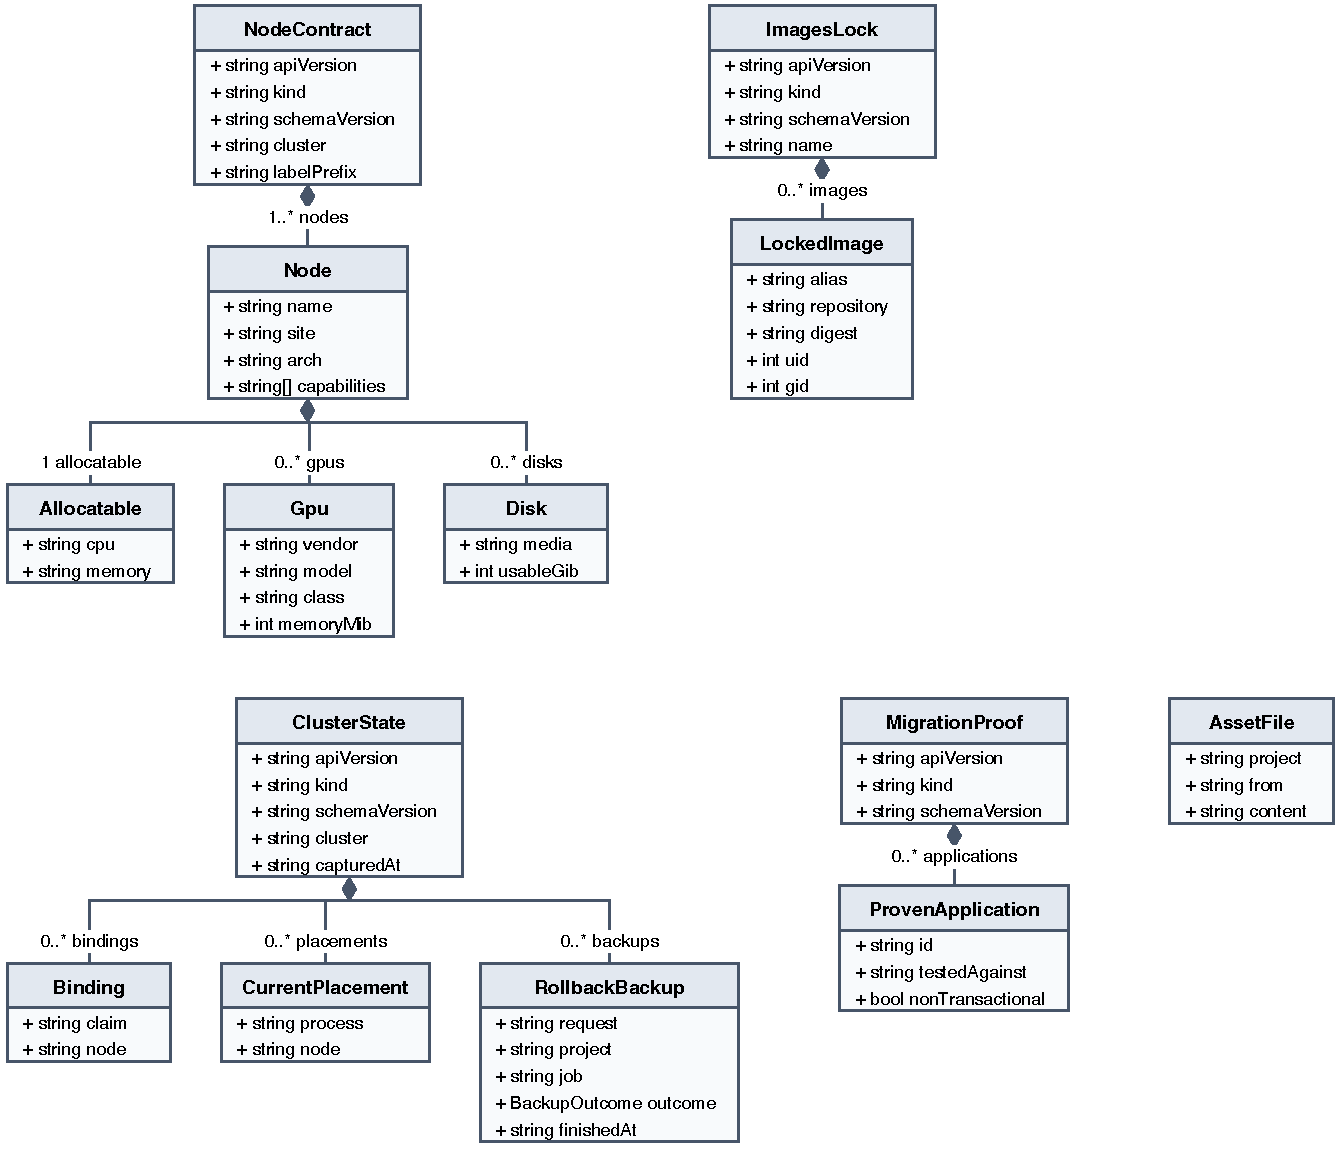
\includegraphics[width=\linewidth, height=0.90\textheight, keepaspectratio]{Figures/pinned-inputs}
\caption{The Pinned Inputs Metamodel. All classes are new; diamonds mark containment}
\label{fig:pinned}
\end{figure}

\begin{figure}[p]
\centering
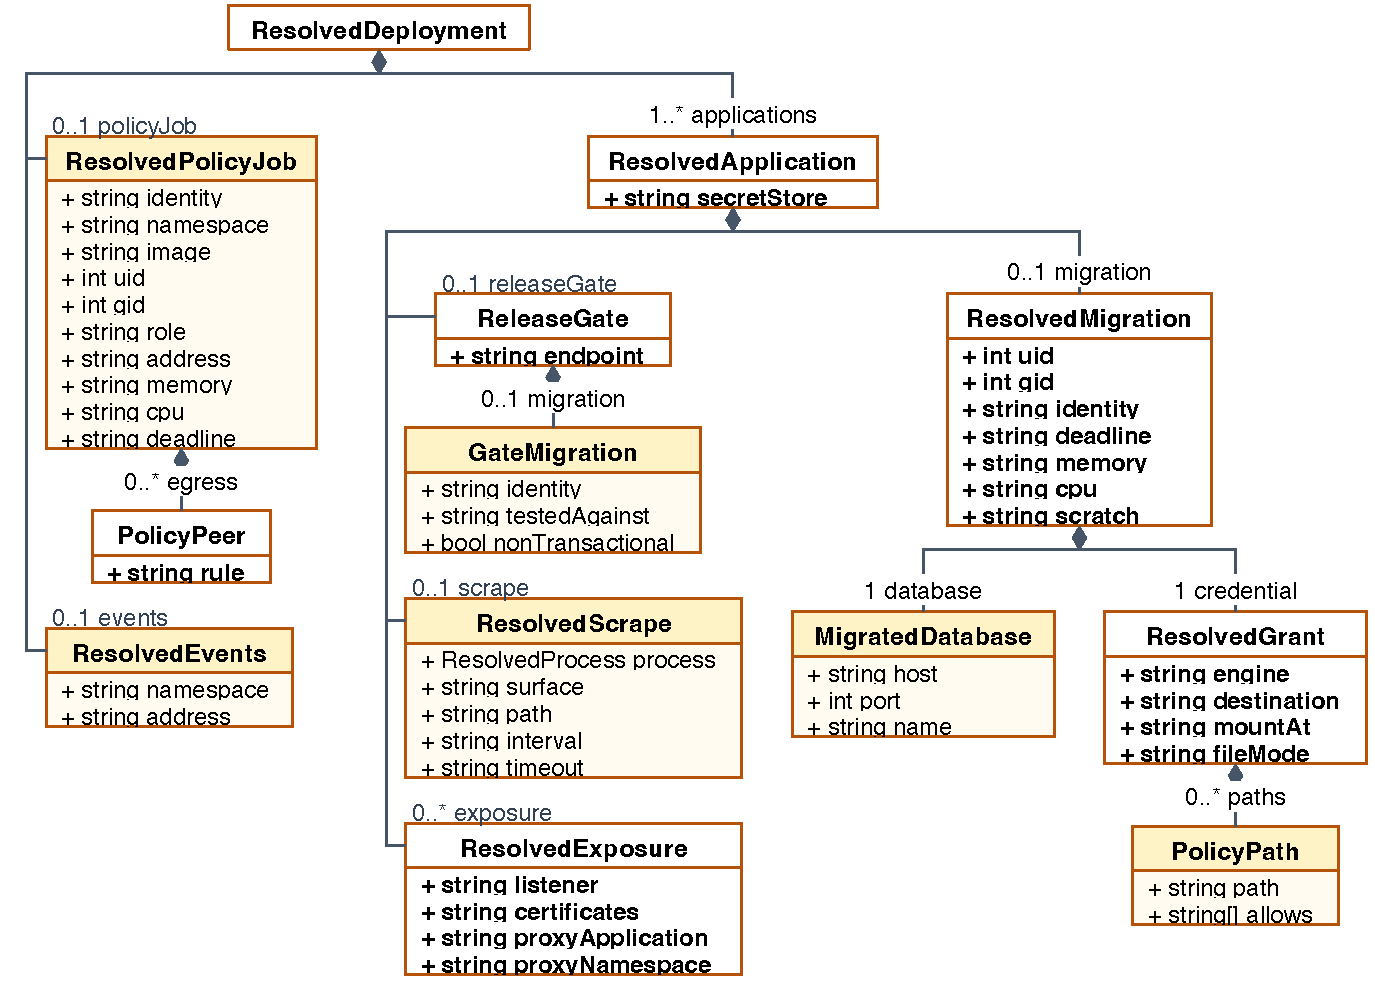
\includegraphics[width=\linewidth, height=0.90\textheight, keepaspectratio]{Figures/target-decisions-application}
\caption{Changed Deployment and Application Classes. Filled classes are new; white Task~1 classes show added features in bold. Diamonds mark containment}
\label{fig:targetdecisions}
\end{figure}

\begin{figure}[p]
\centering
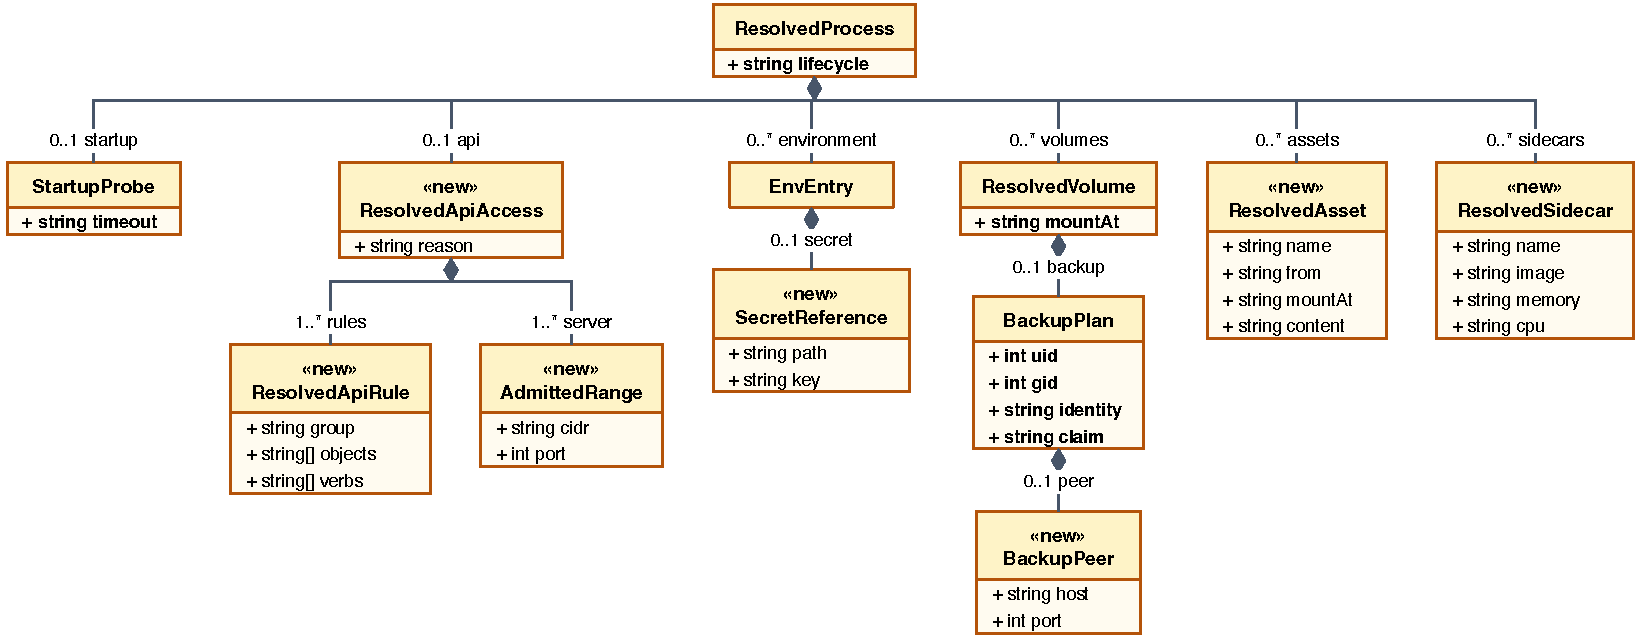
\includegraphics[width=\linewidth, height=0.90\textheight, keepaspectratio]{Figures/target-decisions-process}
\caption{Changed Process and Release Analysis Classes. Parent classes are repeated for context; colours and feature markings follow Figure~\ref{fig:targetdecisions}}
\label{fig:targetprocesses}
\end{figure}

\begin{figure}[p]
\centering
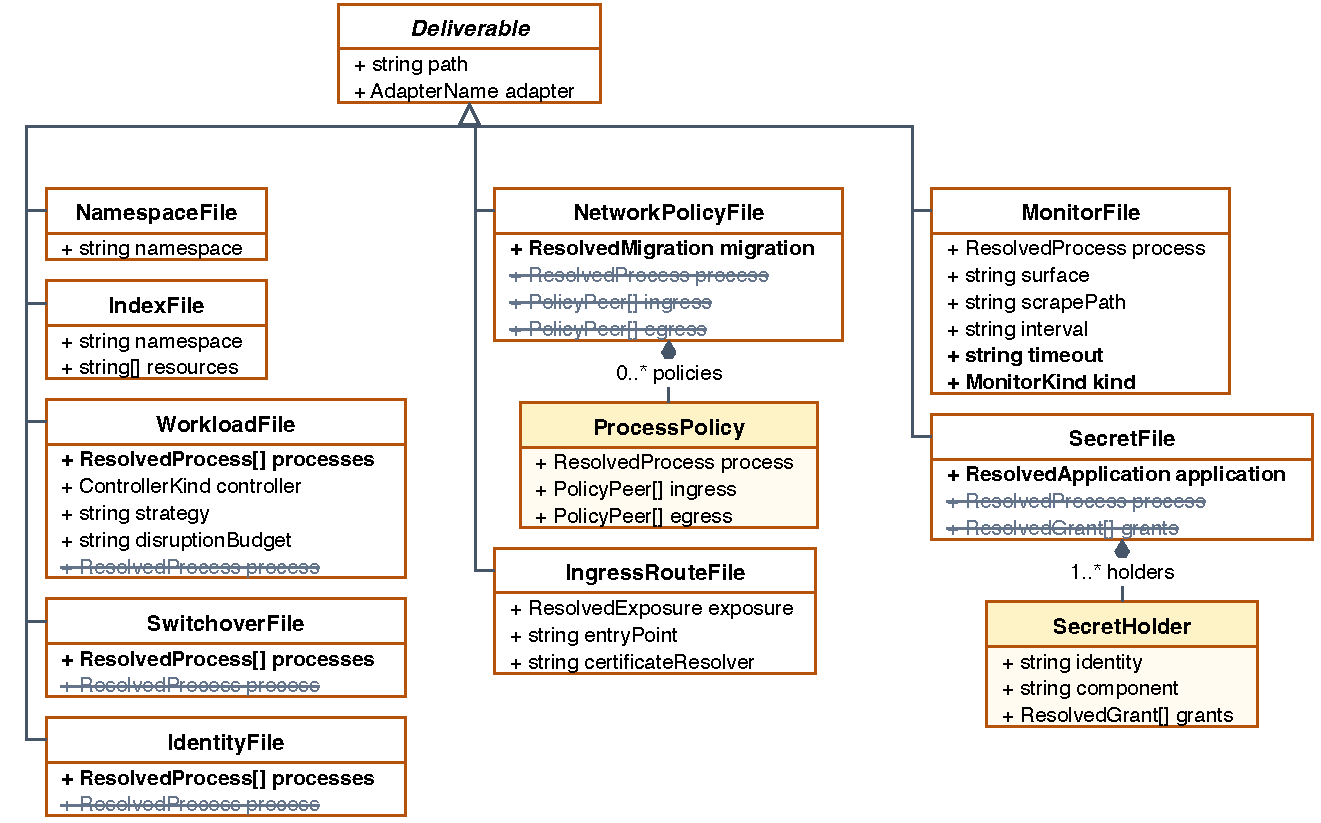
\includegraphics[width=\linewidth, height=0.90\textheight, keepaspectratio]{Figures/target-files-existing}
\caption{Task~1 Generated-File Classes and Their Changes. Bold marks added features; strikethrough marks removed features. Filled helper classes are new}
\label{fig:targetfiles}
\end{figure}

\begin{figure}[p]
\centering
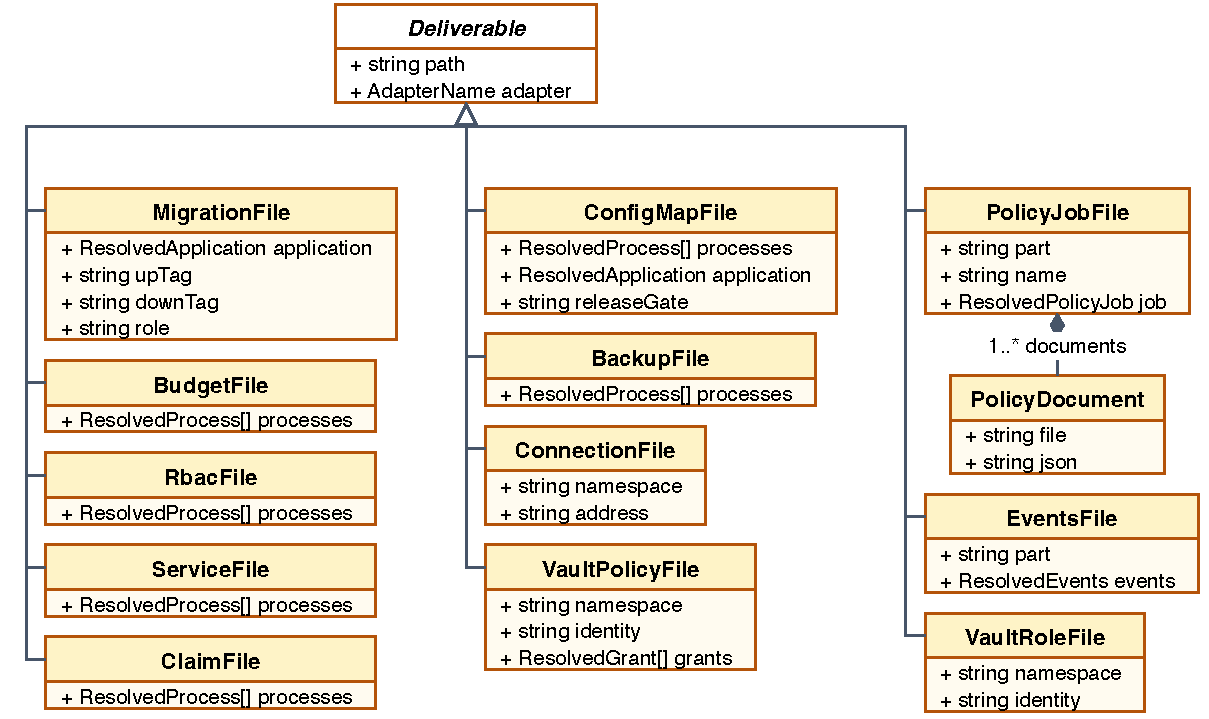
\includegraphics[width=\linewidth, height=0.90\textheight, keepaspectratio]{Figures/target-files-added}
\caption{The Twelve Added Generated-File Classes. The Abstract Deliverable Parent is Repeated for Context; All Classes Belong to the Target Metamodel}
\label{fig:targetfilesadded}
\end{figure}
\end{landscape}

\section{The Hand-in Archive}
\label{app:handin}

The archive holds report.pdf, a README.md with the steps from
Appendix~\ref{app:running}, and two folders.

task-2-transformations/ is an Eclipse project for reading the models
(Table~\ref{tab:handin}), imported via File > Import > Existing Projects
into Workspace. It contains no Java, so the transformations do not run from
it: the resolution and estate pass call the Hashing library, which the
implementation plug-in registers.

implementation/ holds the EMF implementation and the examples the tests read.

\begin{table}[!htbp]
\centering
\begin{tabular}{>{\raggedright\arraybackslash}p{0.5\linewidth}>{\raggedright\arraybackslash}p{0.42\linewidth}}
\hline
\textbf{Path} & \textbf{Contents} \\
\hline
model/ & The source, pinned-inputs and target metamodels. \\
transforms/ & lower.qvto, resolution.qvto and estate.qvto. \\
examples/platform/ & The Platform Intent and the pinned inputs every example reads. \\
examples/<example>/authored/ & The Project Intent with its env and configuration files. \\
examples/<example>/resolution.intent.xmi & The intent extent: authored and lowered Projects, plus Platform Intent. \\
examples/<example>/resolution.pinned.xmi & The pinned extent. \\
examples/<example>/<project>.resolveddeployment & The Resolved Deployment the transformation wrote. \\
examples/<example>/dependencies.json & The edges exported from it, beside expected-dependencies.json, a copy of the oracle expected/dependencies.json. \\
examples/minimal/minimal.hand-written.resolveddeployment & The hand-written target model from Task~1, updated in Appendix~\ref{app:target}. \\
examples/secrets/secrets.expected.resolveddeployment & The complete expected model of secrets (Section~\ref{sec:thin}). \\
\hline
\end{tabular}
\caption{The Models Project of the Archive, One Folder per Example of Table~\ref{tab:results}}
\label{tab:handin}
\end{table}

Every XMI declares its metamodel in xsi:schemaLocation, so Eclipse opens it
in the Sample Reflective Ecore Model Editor without a registered package.

\subsection{Running the Transformations}
\label{app:running}

In implementation/emf, run ./mvnw clean verify with JDK~21. It builds the
implementation, runs every test, and writes each example's models and edges
under bundles/cli/target/parity/<example>/. It takes about 17 seconds.

In Eclipse Modeling Tools with the QVT-Operational SDK, import
implementation/emf as existing Maven Projects.

Run resolution.launch in dev.jorisjonkers.deploykit.emf.resolve. It resolves
minimal from the extents step 1 wrote.


\begin{thebibliography}{9}
\bibitem{kubediagrams} P.~Merle and F.~Petrillo. Visualizing Cloud-native
  Applications with KubeDiagrams. In \emph{Proc.\ VISSOFT 2025}, pp.~106--116,
  2025. Tool: \url{https://github.com/philippemerle/KubeDiagrams}.
\bibitem{kubeorch} KubeOrch, visual Kubernetes workflow orchestrator.
  \url{https://github.com/KubeOrch} (repositories \texttt{core} and
  \texttt{ui}), visited 15 October 2026.
\bibitem{kubert} kubert, a kubectx and kubens alternative.
  \url{https://github.com/idebeijer/kubert}, visited 15 October 2026.
\bibitem{burgueno2019} L.~Burgue\~no, J.~Cabot and S.~G\'erard. The Future of
  Model Transformation Languages: An Open Community Discussion. \emph{Journal of
  Object Technology} 18(3), 7:1--11, 2019.
\bibitem{amstel2011} M.~van Amstel, S.~Bosems, I.~Kurtev and L.~Ferreira Pires.
  Performance in Model Transformations: Experiments with ATL and QVT. In
  \emph{Proc.\ ICMT 2011}, LNCS 6707, pp.~198--212, 2011.
\bibitem{qvt13} Object Management Group. \emph{Meta Object Facility
  Query/View/Transformation Specification}, version 1.3, 2016.
\end{thebibliography}

%==== END OF ALL ===
\end{document}
